\documentclass[12pt]{report}
\usepackage{amsmath}
\usepackage{graphicx}
\def\figdir{mfigs}
\begin{document}


\title{\Huge\bf Material inversion with SW4mopt} 

\author{Bj\"orn Sj\"ogreen$^1$ \and N. Anders Petersson\thanks{Center for Applied Scientific
     Computing, Lawrence Livermore National Laboratory, PO Box 808, Livermore CA 94551.}}
\date{September 27, 2013} 
\maketitle



%-----------------------------------------------------------------------
\chapter{ Introduction }\label{sec:matopt}

\emph{SW4mopt} is a solver for material inversion and source inversion, built on
the forward solver \emph{SW4}. Running \emph{SW4mopt} is very similar to running
\emph{SW4}. \emph{SW4mopt} uses the same input commands as \emph{SW4}, and 
provides an extended set of commands, related to the inverse problem.
\par
Given time series data at a number of stations, \emph{SW4mopt} solves for the material
density, $\rho$, and Lam\'e parameters $\mu$ and $\lambda$, in
a material that has been parameterized in some way. Currently, the only available parameterization
is a representation of the material on a coarse grid. The material at the grid points is 
defined by interpolation from this coarse grid. \emph{SW4mopt} is written such that it will
be easy to extend to other types of parameterizations, e.g., representation as B-splines or 
a mesh free unstructured representation.
\par
For minimization, \emph{SW4mopt} provides the choice of the limited memory BFGS method (L-BFGS)
or a non-linear conjugate gradient method. These are run together with a line search algorithm
to determine the step length. 
\par
As of writing, September 2013, \emph{SW4mopt} has been successfully run on simple problems 
with synthetic data, some of them reported below. It is a complete solver for the inverse problem. 
However, it is far from being ready to be released to the users. \emph{SW4mopt} is not as 
robust as \emph{SW4}, and we need to test it on many other problems, to make sure that it works 
as expected, and to gain experience of material inversion. Furthermore, since \emph{SW4mopt} is 
still in development, it produces a lot of output messages that might be confusing to the average user.

The following should be done to improve \emph{SW4mopt}.
\begin{itemize}
\item Implement the material parameterization for grids with topography. Topography is the only critical
      part that is missing. The material gradient can be computed with topography, it is just the
      coarse grid parameterization that has not been done.
\item Implement a material parameterization which is distributed on the processors. Currently one copy of
      the entire coarse material grid is stored in each processor. This will lead to memory limitations
      as problems size increases. 
\item Possibility to refine the material grid, so that the inversion to a highly resolved material can 
      be made hierarchally. The same
      holds for the scaling factors. With a higher material resolution, we can not expect to compute these
      by forming the Hessian. Can scaling factors be interpolated from a coarse grid inversion ?
\item Automatic readjustment of the time step when the material speed increases past the 
      largest stable CFL number. This must now be handled by manual restart, it would be better to have
      the code doing it automatically.
\end{itemize}
\par
A few more items that should be addressed, but which require new research and development,
and new software.
\begin{itemize}
\item Material inversion in an anisotropic material.
\item Homogenization techniques to recover isotropic material properties from the result of 
      anisotropic material inversion.
\item Material inversion with attenuation.
\end{itemize}





%-----------------------------------------------------------------------
\chapter{The material description}\label{sec:matdesc}



\section{The mparcart command}\label{sec:mparcartdesc}

The \verb+mparcart+ defines a material that is discretized on a coarse Cartesian grid, 
below refered to as the ``material grid''. The parameters are the offset values of 
$\rho$, $\mu$, and $\lambda$ relative a reference material, at the points of this grid. 
The material on the computational grid 
is defined by trilinear interpolation from the values on the coarser material grid. 
For example, the density, $\rho$, at a grid point $(i,j,k)$ in the computational grid is 
$$
  \rho_{i,j,k} = I(\{d^{(\rho)}\},x_i,y_j,z_k) + \rho^{(0)}_{i,j,k}
$$
where $\rho^{(0)}$ is the reference material, and $d^{(\rho)}$ is the difference $\rho-\rho^{(0)}$ 
on the material grid. The interpolation operator
$$
 I(\{ u \}, x,y,z)
$$
evaluates a function $u$ defined at the points of the material grid, at the point $(x,y,z)$.
\par
The number of points in the material grid, and initial values for $d^{(\rho)}, d^{(\mu)}, d^{(\lambda)}$
are specified by the \verb+mparcart+ command. For example
\begin{verbatim}
mparcart nx=5 ny=5 nz=3 init=0
\end{verbatim}
defines a material grid with $5\times 5\times 3$ points, and with $d^{(\rho)}$, $d^{(\mu)}$, $d^{(\lambda)}$
initialized to zero at all points.
The reference material is specified by one of the material commands 
of \emph{SW4}, e.g., \verb+block+ or \verb+pfile+, see the \emph{SW4} User's Guide for a
complete description of these material commands.

\par
Using a coarse material grid reduces the number of unknowns, compared with using the 
material at each grid point as parameters. Furthermore, the resolution in the material
is limited in terms of highest frequencies of the computed wave field, making it unreasonable
to expect to resolve the material down to the resolution of the computational grid.
We recommend that the grid spacing of the material grid is around 10 times 
the grid spacing of the computational grid. Also to note, the grid spacing of the material 
grid do not need to have any relation to the spacing of the computational grid. 
These two grids are independent.
\par
\begin{figure}
\begin{center}
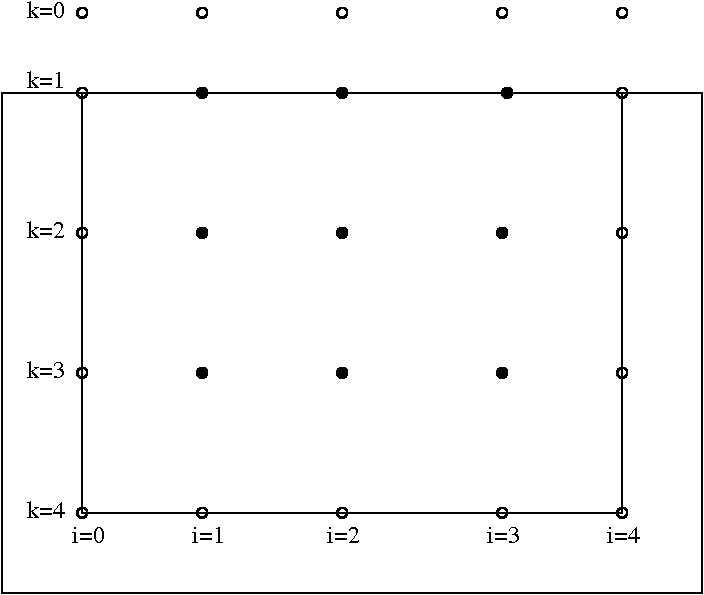
\includegraphics[width=0.8\textwidth]{\figdir/mparcart.png}
\caption{Two dimensional slice of a material grid with $n_x=n_y=n_z=3$. The free surface boundary
is at $k=1$, there are super-grid sponge layers on the other sides. Filled circles indicate unknown
parameters, open circles are fixed boundary values.}
\label{fig:mparcart}
\end{center}
\end{figure}
\par
The material grid discretizes only the interior part the domain, without the super-grid
sponge layers. The configuration is outlined in Fig.~\ref{fig:mparcart}.
The material grid is given by
\begin{alignat}{2}
 x_i = x_{min}+ i h_x \qquad i=0,\ldots,n_x+1\\
 y_j = y_{min}+ j h_y \qquad j=0,\ldots,n_y+1\\
 z_k = z_{min}+ k h_z \qquad k=0,\ldots,n_z+1
\end{alignat}
where the grid spacings $h_x$, $h_y$, and $h_z$ are determined such that $x_0, y_0, x_{n_x+1}, y_{n_y+1}$,
and $z_{n_z+1}$ are located at the interface between the interior domain and the super-grid sponge layer. 
In the depth direction, $z_1$ is on the free surface and, hence $z_{min}=-h_z$. The point $z_0$ is above the 
topography, but it will never be used in the interpolation. 

At the first and last points in each direction, ($i=0$, $j=0$, $k=0$, $n_x+1$, $n_y+1$, and $n_z+1$),
the offsets $d^{(\rho)}, d^{(\mu)}$, and $d^{(\lambda)}$ are fixed at zero, hence these values are
not part of the parameter vector. The total number of unknowns for the material inversion
is $3 \times n_x \times n_y \times n_z$.


%-----------------------------------------------------------------------
\chapter{Computed examples}

\section{Material grid with a single point}
This test problem is defined on a domain of size $35000\times 35000\times 17000$.
The material is constant with $\rho=2650$, $v_s=2437.56$, and $v_p=4630.76$, giving
$\mu=1.57455\times 10^{10}$ and $\lambda=2.5335\times 10^{10}$. The elastic wave equation 
is discretized on a grid with spacing $h=200$. A traction free boundary condition is 
imposed at the boundary $z=0$. All other boundaries have super-grid sponge layers of width $2500$.
Waves are set off by a moment source located at $x_s=y_s=17500$, $z_s=2000$. The only
non-zero element of the moment tensor is $M_{xy}=1.0\times 10^{18}$. The source time function
is a Gaussian with $t_0=1.5$ and $\omega=4$.
\par
We consider a material grid of size $1\times 1 \times 1$, i.e., there is only one point
in the material parameterization. 
The total number of material parameters is 3, i.e., $\rho$, $\mu$, and $\lambda$ at the 
single point. The outline of the material grid in Fig.~\ref{fig:mparcart} shows that with
a single point, it will be located at $x=y=17500$ and $z=0$.
\par
Synthetic seismograms are computed at stations on a centered $5\times 5$ grid with spacing $3000$ 
on the surface, ($z=0$). These seismograms, computed with the constant material, are used as the
measured data in the numerical experiments.
In these experiments, we initialize the values at the material grid point by a perturbation
of the constant material. Denoting the constant, reference, density by $\rho^{(ref)}$, and the perturbation
by $d^{(\rho)}$, we have
$$
  \rho    = \rho^{(ref)}+d^{(\rho)}
$$
at the material grid point. The notation for $\mu$ and $\lambda$ are similar.
The following five initial perturbations are considered
\begin{center}
\begin{tabular}{|l|l|l|l|l|} \hline
{\bf Name} & $d^{(\rho)}$ & $d^{(\mu)}$ & $d^{(\lambda)}$  \\ \hline 
pp10 & $0.1\rho^{(ref)}$ & $0.1\mu^{(ref)}$ & $0.1\lambda^{(ref)}$ \\ \hline
mm10 & $-0.1\rho^{(ref)}$ & $-0.1\mu^{(ref)}$ & $-0.1\lambda^{(ref)}$ \\ \hline
mp10 & $-0.1\rho^{(ref)}$ & $0.1\mu^{(ref)}$ & $0.1\lambda^{(ref)}$ \\ \hline
mp30 & $-0.3\rho^{(ref)}$ & $0.3\mu^{(ref)}$ & $0.3\lambda^{(ref)}$ \\ \hline
pm30 & $0.3\rho^{(ref)}$ & $-0.3\mu^{(ref)}$ & $-0.3\lambda^{(ref)}$ \\ \hline
\end{tabular}
\label{tab:cases}
\end{center}
The minimizing algorithm should converge to the constant material, i.e., $d^{(\rho)}$ should approach
zero. The Hessian at the constant material is 
$$
H= \begin{pmatrix}    2.9371e-03 &  -4.9563e-10 & -1.8236e-12 \\
                     -4.9563e-10 &  8.7013e-17  & 2.4771e-19 \\
                     -1.8236e-12 &  2.4771e-19  & 3.6478e-20
   \end{pmatrix}
$$
The condition number of $H$ is $8.571\times 10^{16}$.  
The scale factors obtained from the diagonal elements of $H$, and rescaled to have $s_{\rho}=\rho^{(ref)}$
are,
$$
 s_{\rho} =2650\quad s_\mu = 1.54\times 10^{10}\quad  s_\lambda = 7.52\times 10^{11}
$$
with these scale factors, the condition number is $107$. Note that $s_\rho$ and $s_\mu$ are typical sizes 
of $\rho^{(ref)}$ and $\mu^{(ref)}$ respectively, while $s_\lambda$ is around 30 times larger 
than $\lambda^{(ref)}$.
As an illustration, Fig.~\ref{fig:images} shows the density on the plane $x=17500$ after 1, 2, 3, and 4 iteration
with the L-BFGS method. The initial perturbation at the single material grid point gives a hat shaped initial 
material. The perturbation disappears as the minimizing iterations converges to the constant material 
used to compute the synthetics.
\begin{figure}
\begin{center}
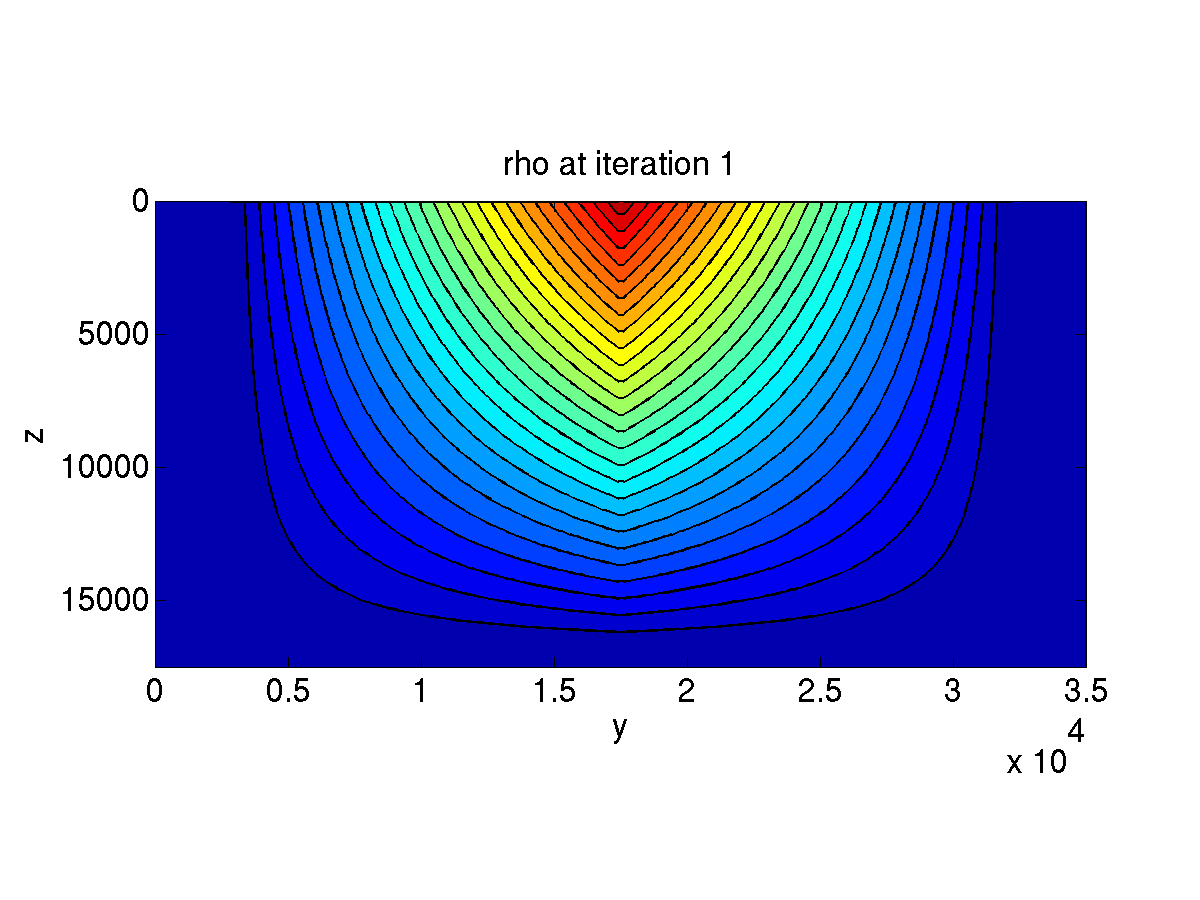
\includegraphics[width=0.45\textwidth]{\figdir/rho-it1-run6.png}\hfil
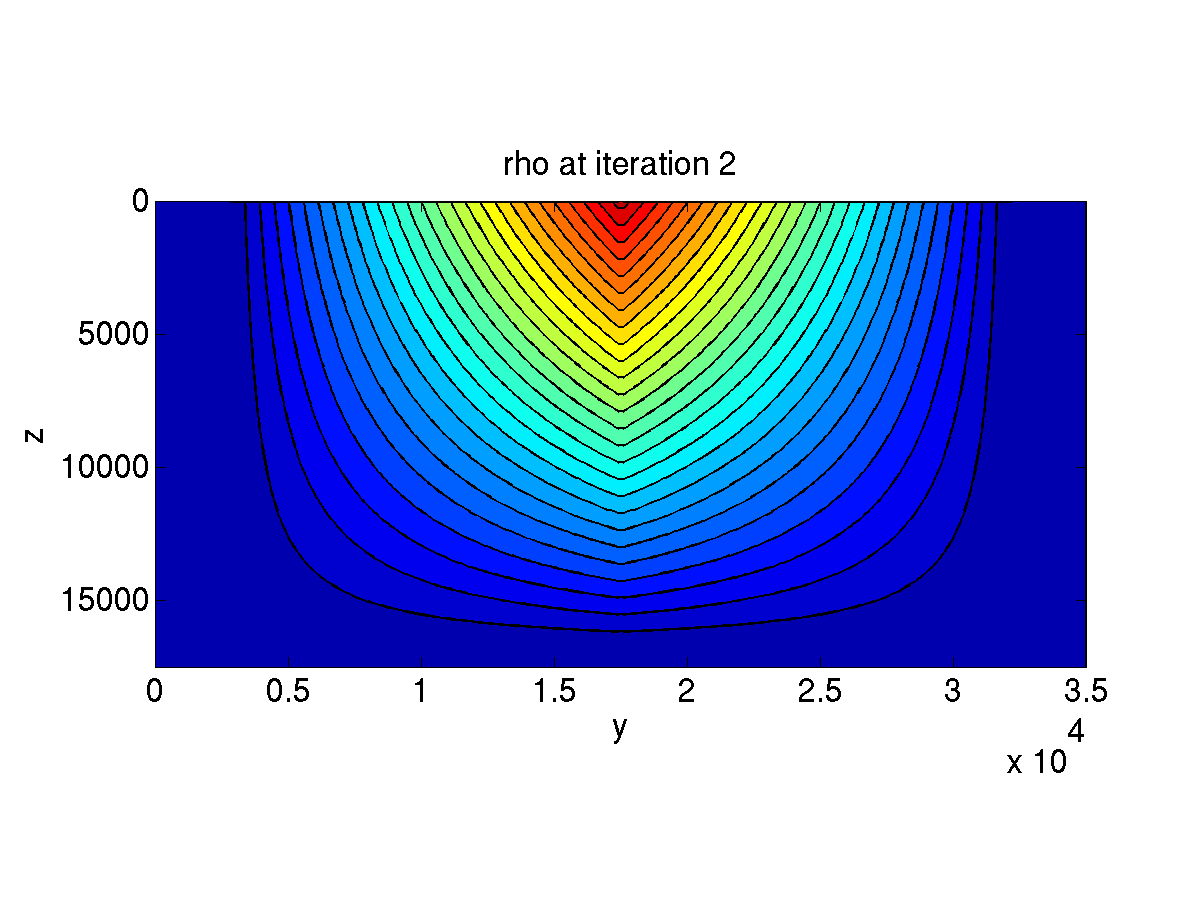
\includegraphics[width=0.45\textwidth]{\figdir/rho-it2-run6.png}\hfil \\
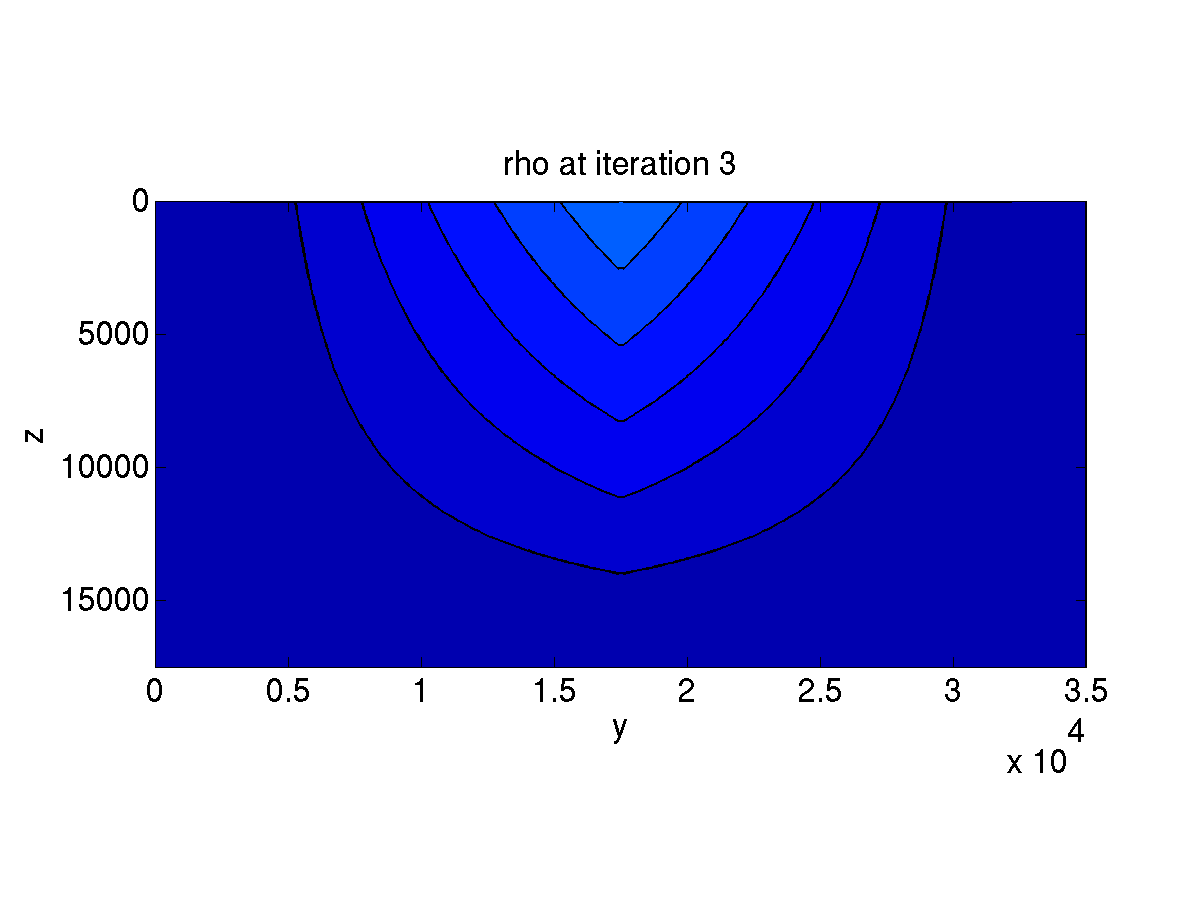
\includegraphics[width=0.45\textwidth]{\figdir/rho-it3-run6.png}
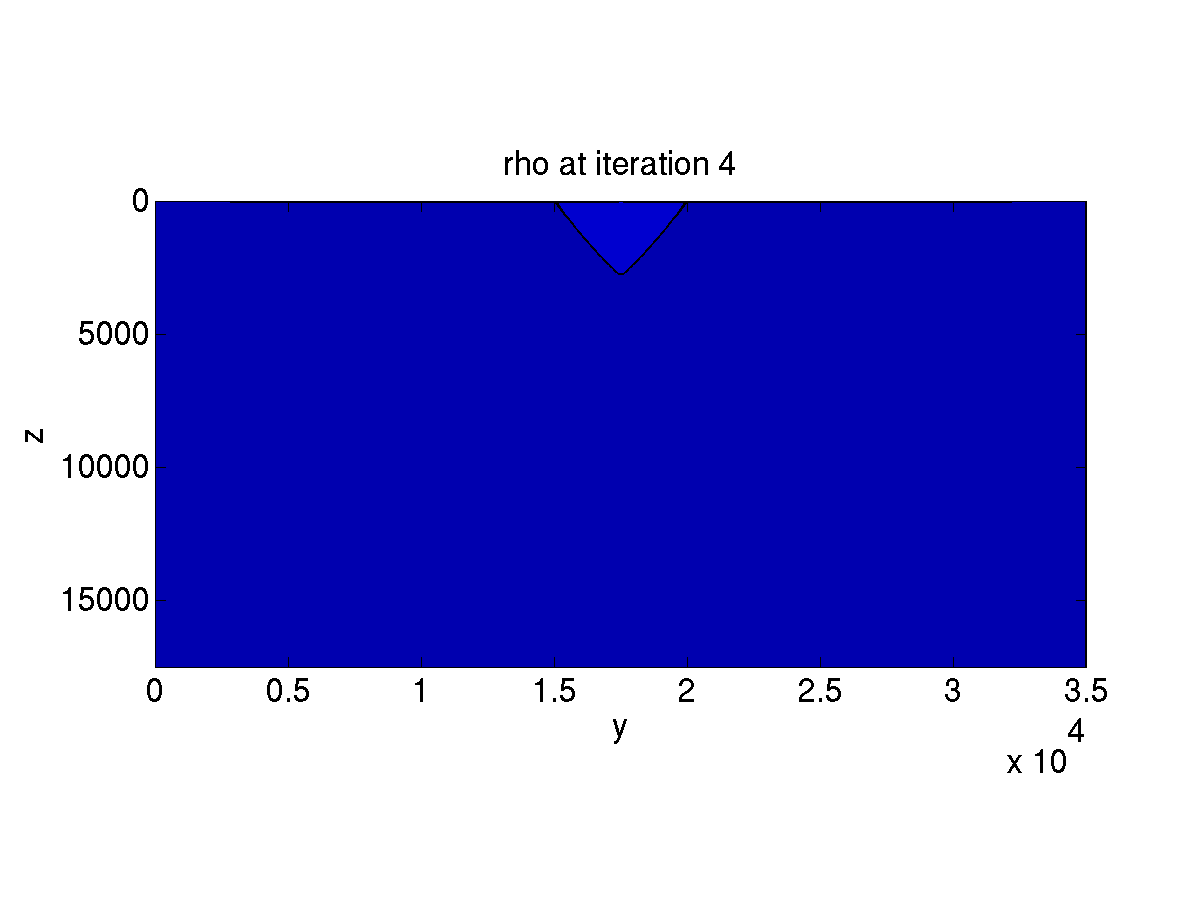
\includegraphics[width=0.45\textwidth]{\figdir/rho-it4-run6.png}
\caption{Density at $x=17500$ after iterations 1, 2, 3, and 4. 30 contour levels between 2650 and 2925.}
\label{fig:images}
\end{center}
\end{figure}
Figure~\ref{fig:per10conv} shows the convergence histories for the cases in Table~\ref{tab:cases} 
with 10\% perturbation. The convergence from the 30\% perturbation are shown in Fig.~\ref{fig:per30conv}.
\begin{figure}
\begin{center}
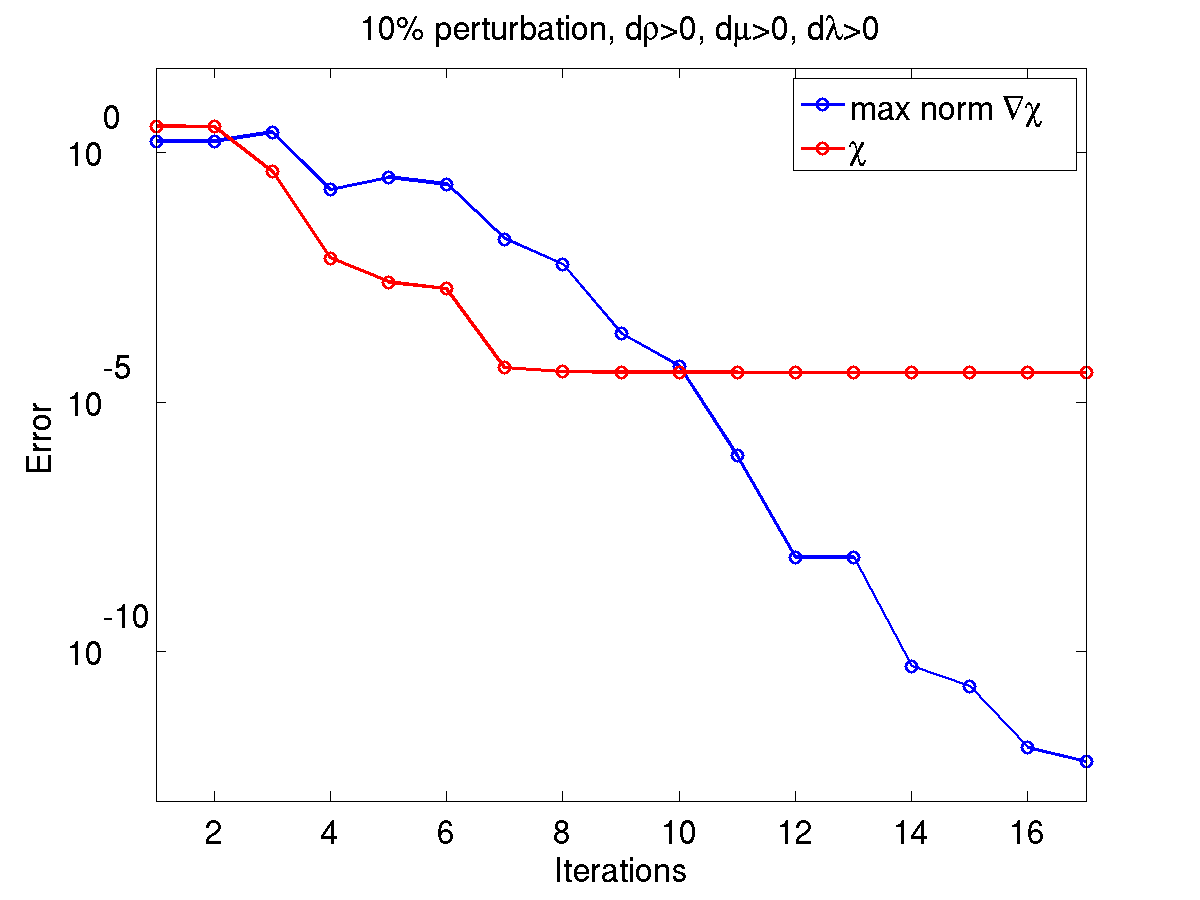
\includegraphics[width=0.33\textwidth]{\figdir/per10pp-conv-m.png}\hfil
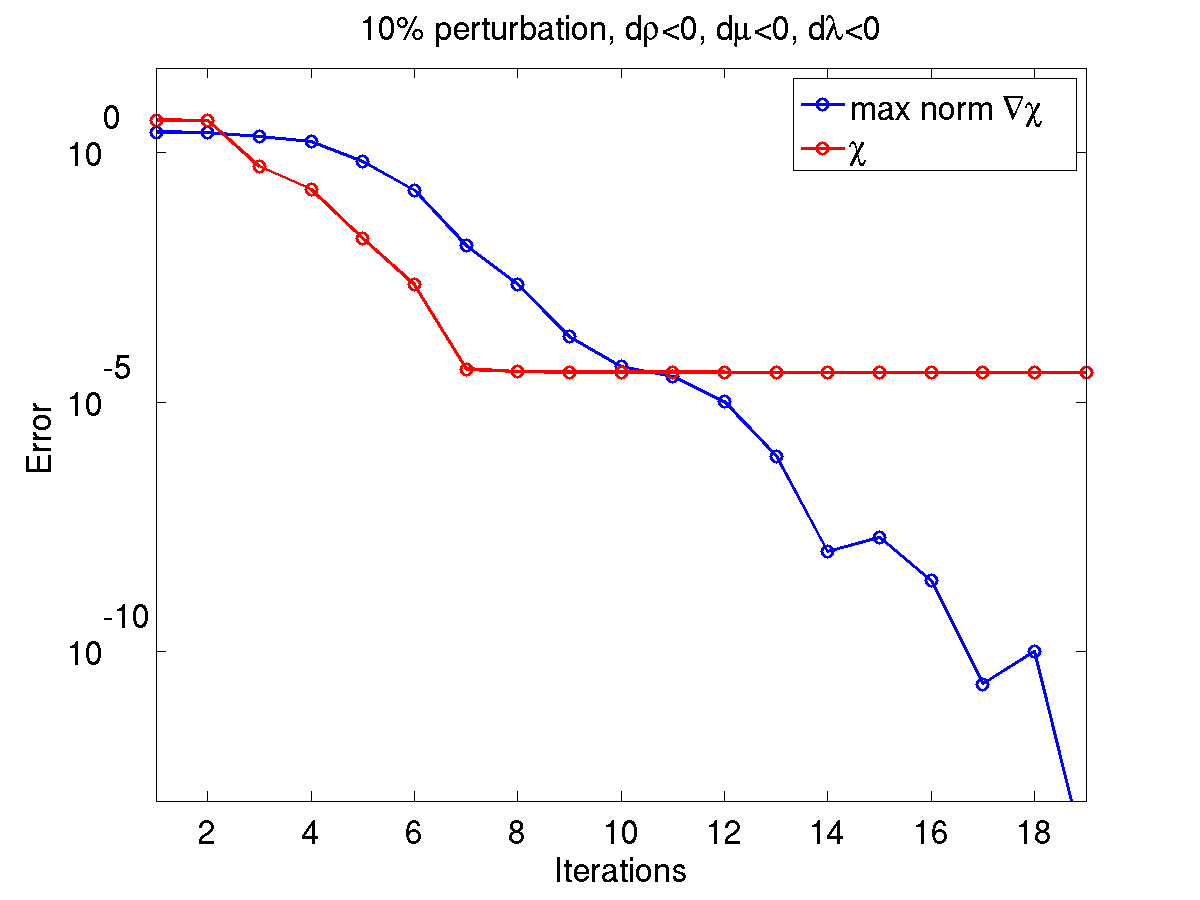
\includegraphics[width=0.33\textwidth]{\figdir/per10mm-conv-m.png}\hfil
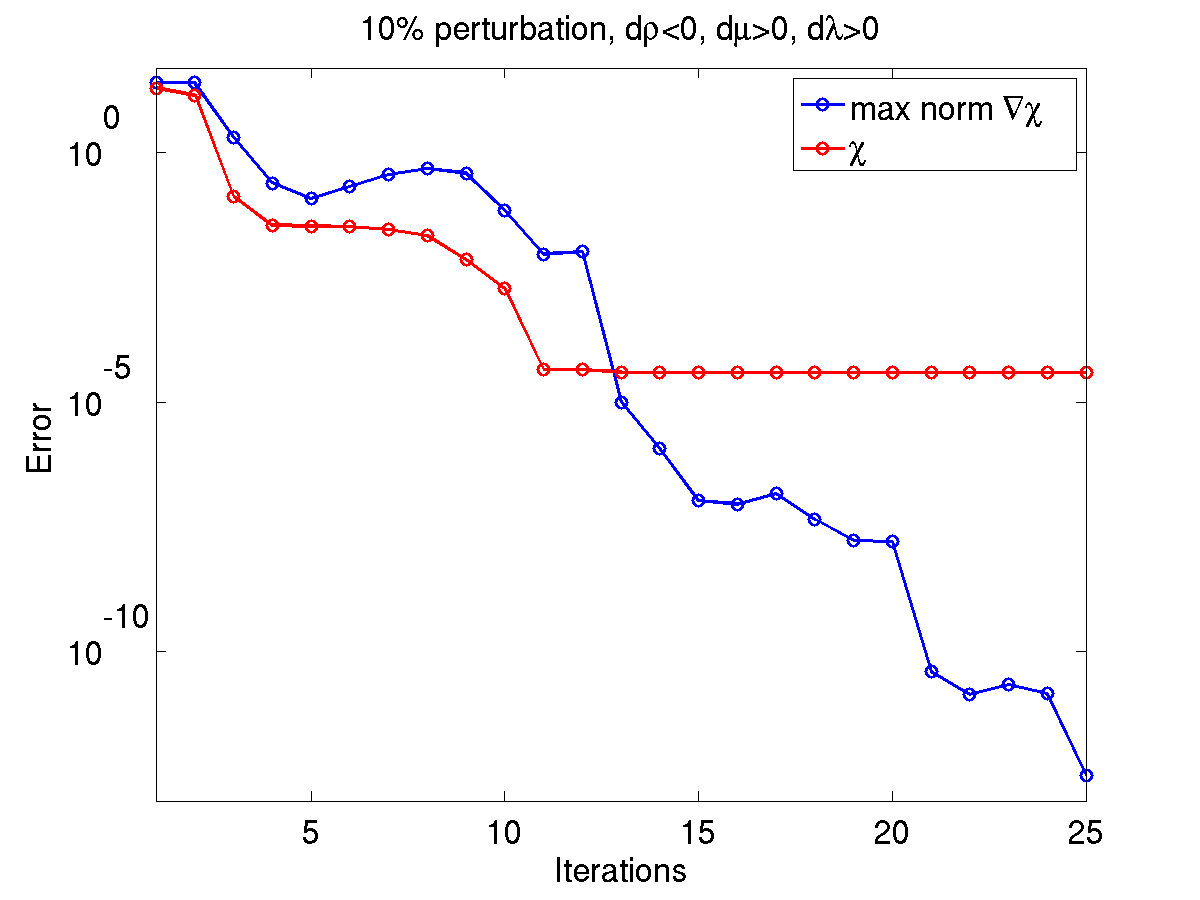
\includegraphics[width=0.33\textwidth]{\figdir/per10mp-conv-m.png}
\caption{Convergence rate of problems pp10 (left), mm10 (middle), and mp10 (right). Blue
is the maximum norm of the gradient of the misfit, red is the misfit.}
\label{fig:per10conv}
\end{center}
\end{figure}

\begin{figure}
\begin{center}
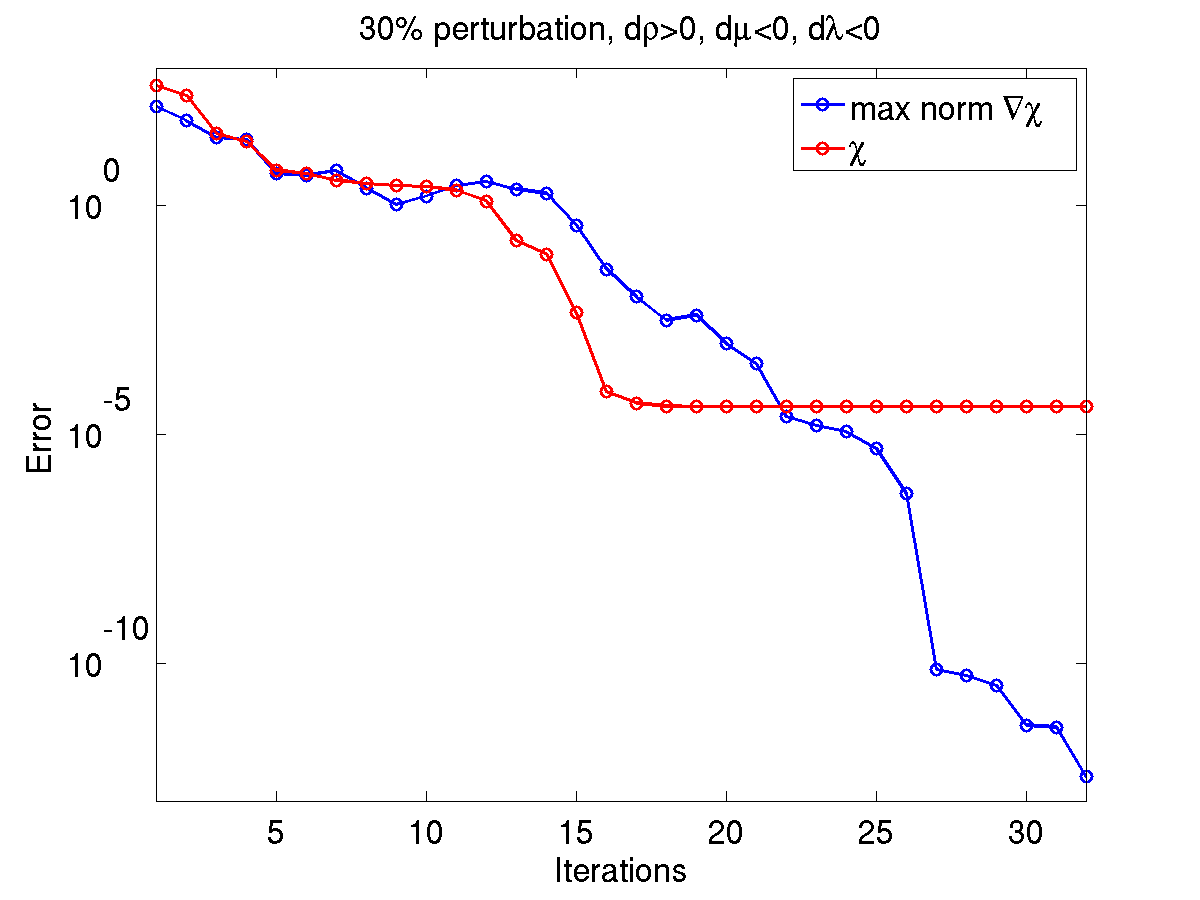
\includegraphics[width=0.45\textwidth]{\figdir/per30pm-conv-m.png}\hfil
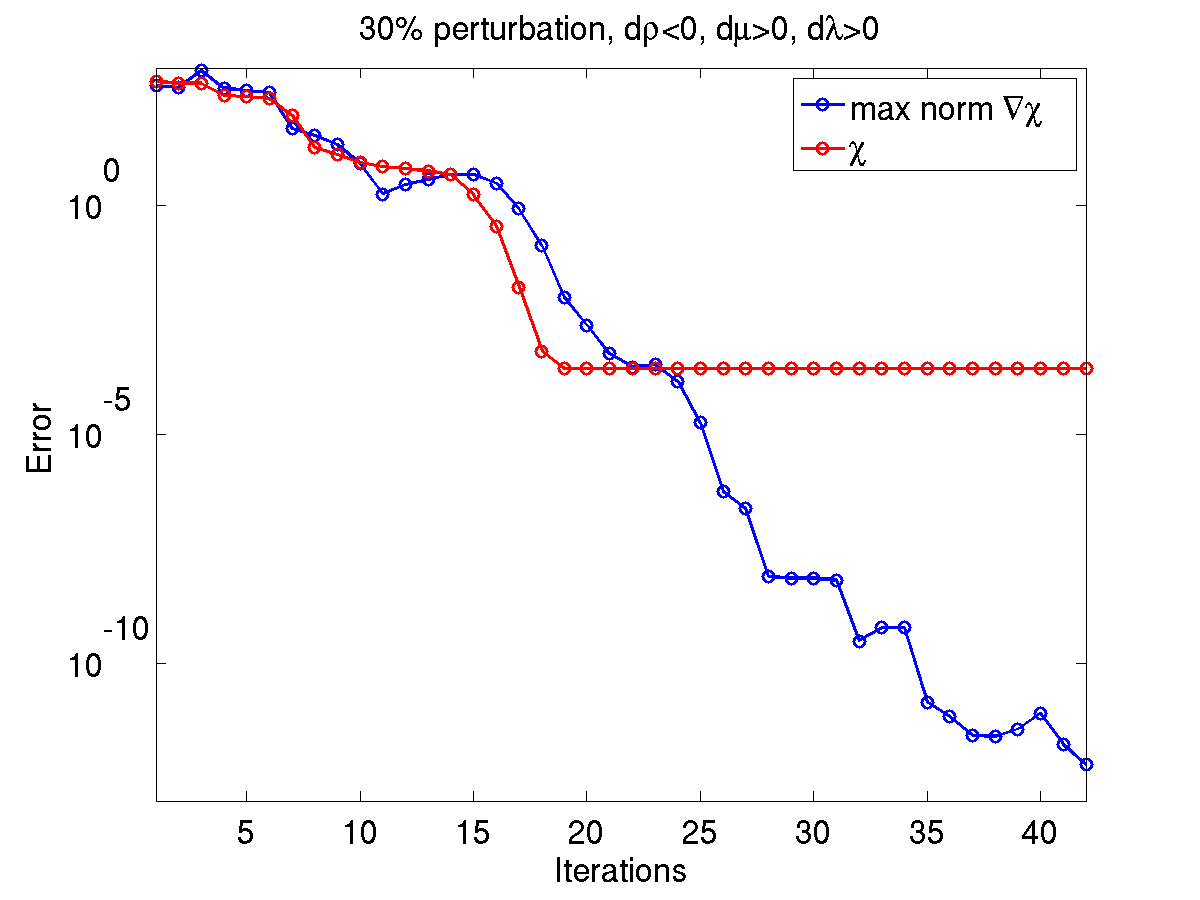
\includegraphics[width=0.45\textwidth]{\figdir/per30mp-conv-m.png}
\caption{Convergence rate of problems pm30 (left), mp30 (right). Blue
is the maximum norm of the gradient of the misfit, red is the misfit.}
\label{fig:per30conv}
\end{center}
\end{figure}
With the 10\% perturbation, it takes 7-10 iterations to converge the misfit down 
to its final value. The 30\% perturbations require 17-20 iterations. 
\par
Next, we investigate the convergence of the material properties at the material grid point.
Figures~\ref{fig:per10vars} and \ref{fig:per30vars} show the evolution of the 
relative error, $d^{(\rho)}/\rho^{(ref)}$ for the density and similarly for $\mu$ and $\lambda$.
The perturbation converges to zero, and as shown by the convergence curves, the material has
converged in the picture norm after around 10 iterations for the 10\%  perturbations. With the
30\% initial perturbation, around 20 iterations are needed. Figures~\ref{fig:per10vars} and \ref{fig:per30vars}
also show that the amplitudes of the perturbations in $\rho$ and $\mu$ never exceeds the size of the
initial perturbation. $\lambda$, on the other hands, have very large variation, especially for the 30\%
perturbation. This is caused by the scaling factor $s_\lambda$ being much larger than the 
size of $\lambda^{(ref)}$. The line search algorithm bases its largest allowed step length on the scale
factors, which implies that a much longer relative step is allowed for $\lambda$ than for $\rho$ and $\mu$.

\begin{figure}
\begin{center}
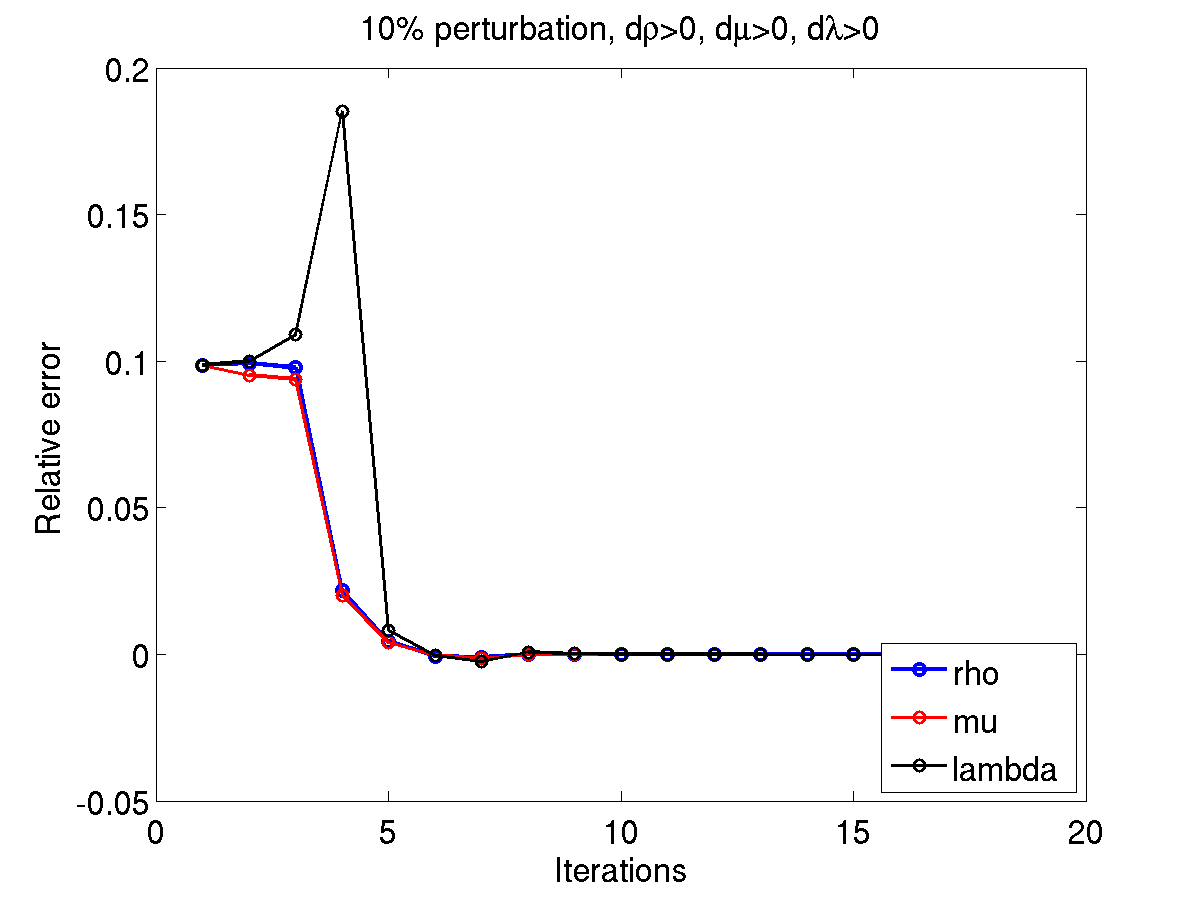
\includegraphics[width=0.33\textwidth]{\figdir/per10pp-m.png}\hfil
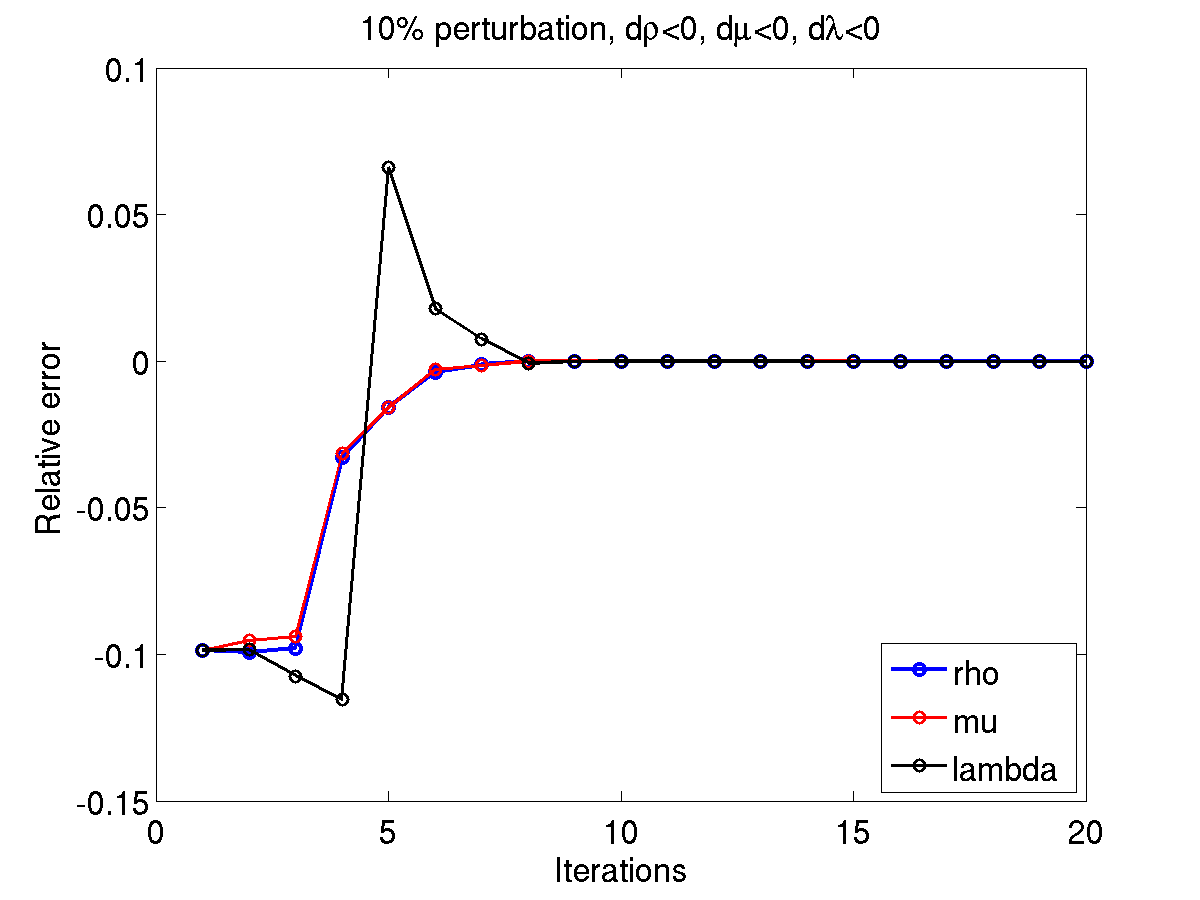
\includegraphics[width=0.33\textwidth]{\figdir/per10mm-m.png}\hfil
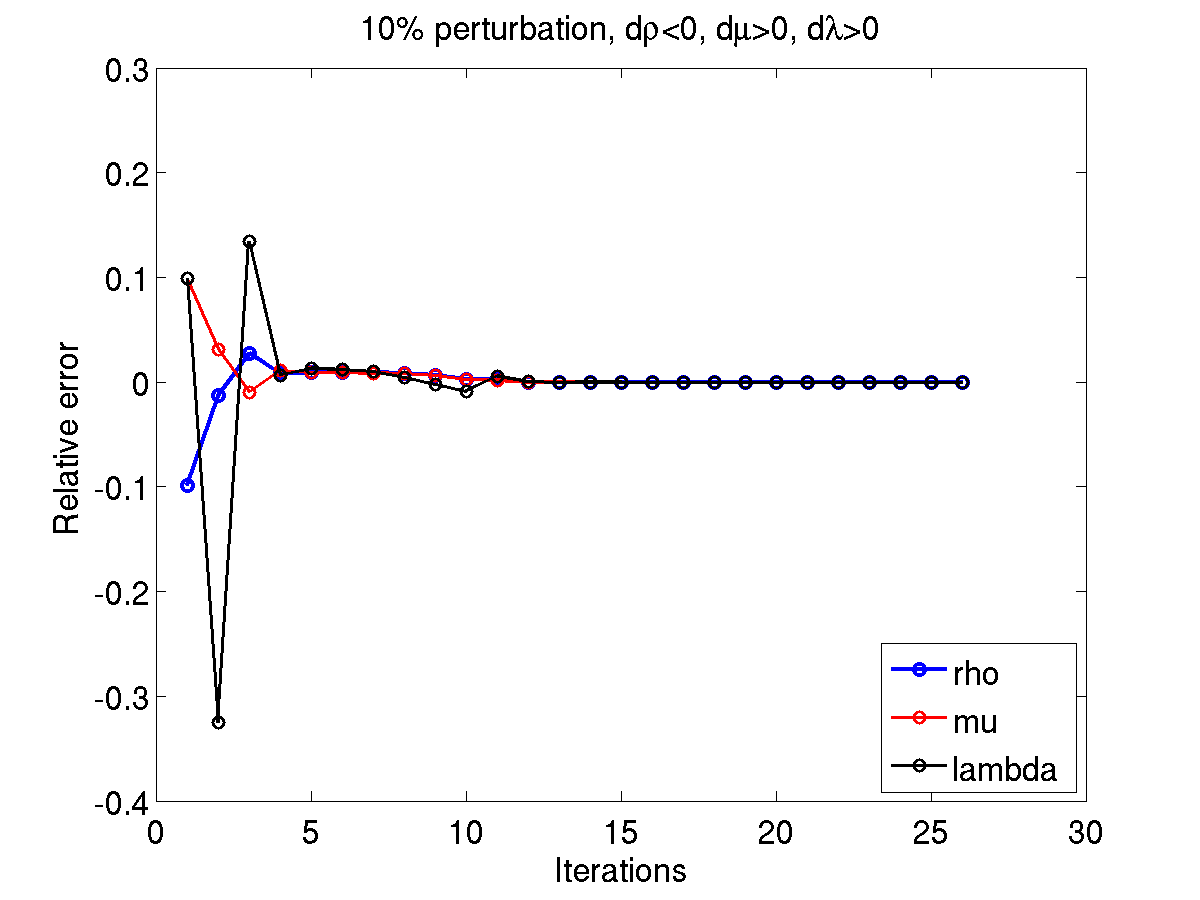
\includegraphics[width=0.33\textwidth]{\figdir/per10mp-m.png}
\caption{Convergence of $\rho$ (blue), $\mu$ (red), and $\lambda$ (black) for 
problems pp10 (left), mm10 (middle), and mp10 (right).}
\label{fig:per10vars}
\end{center}
\end{figure}

\begin{figure}
\begin{center}
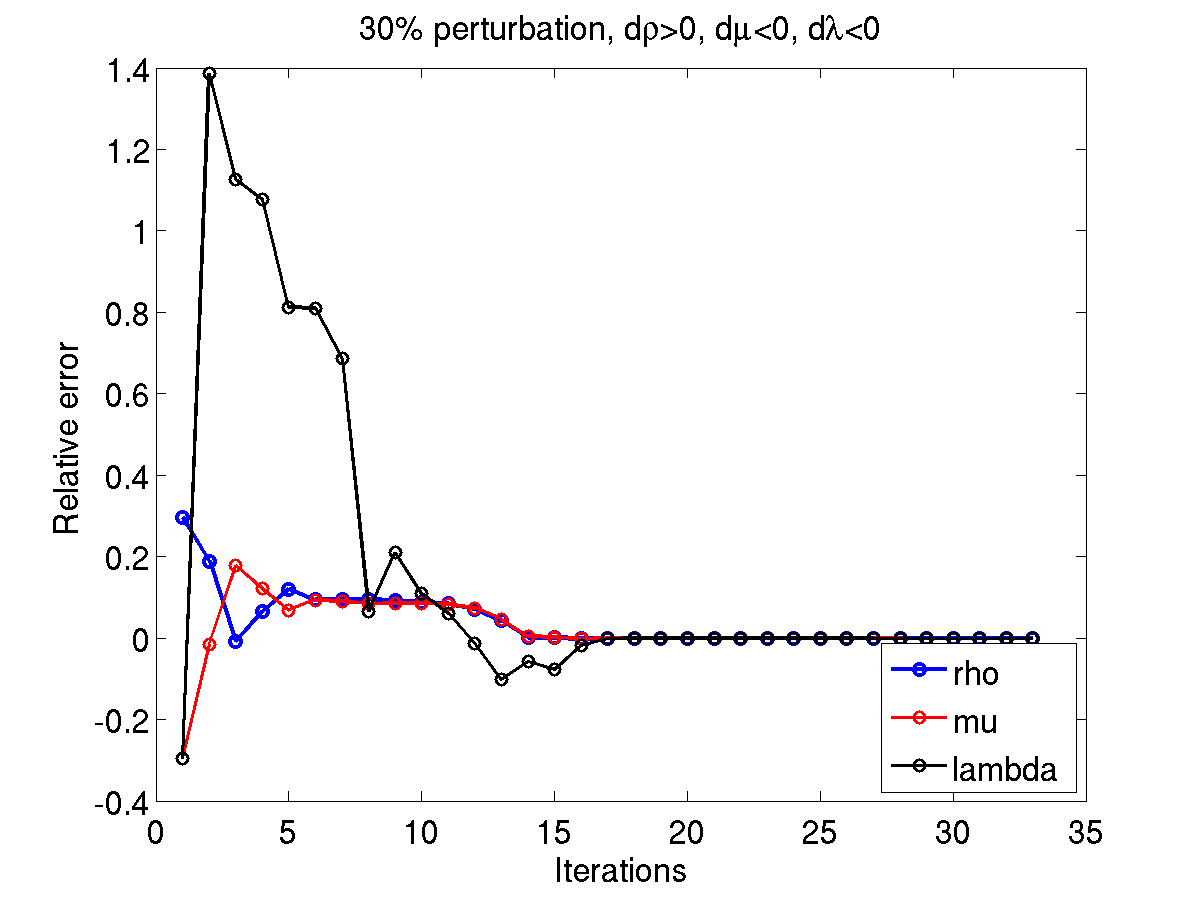
\includegraphics[width=0.45\textwidth]{\figdir/per30pm-m.png}\hfil
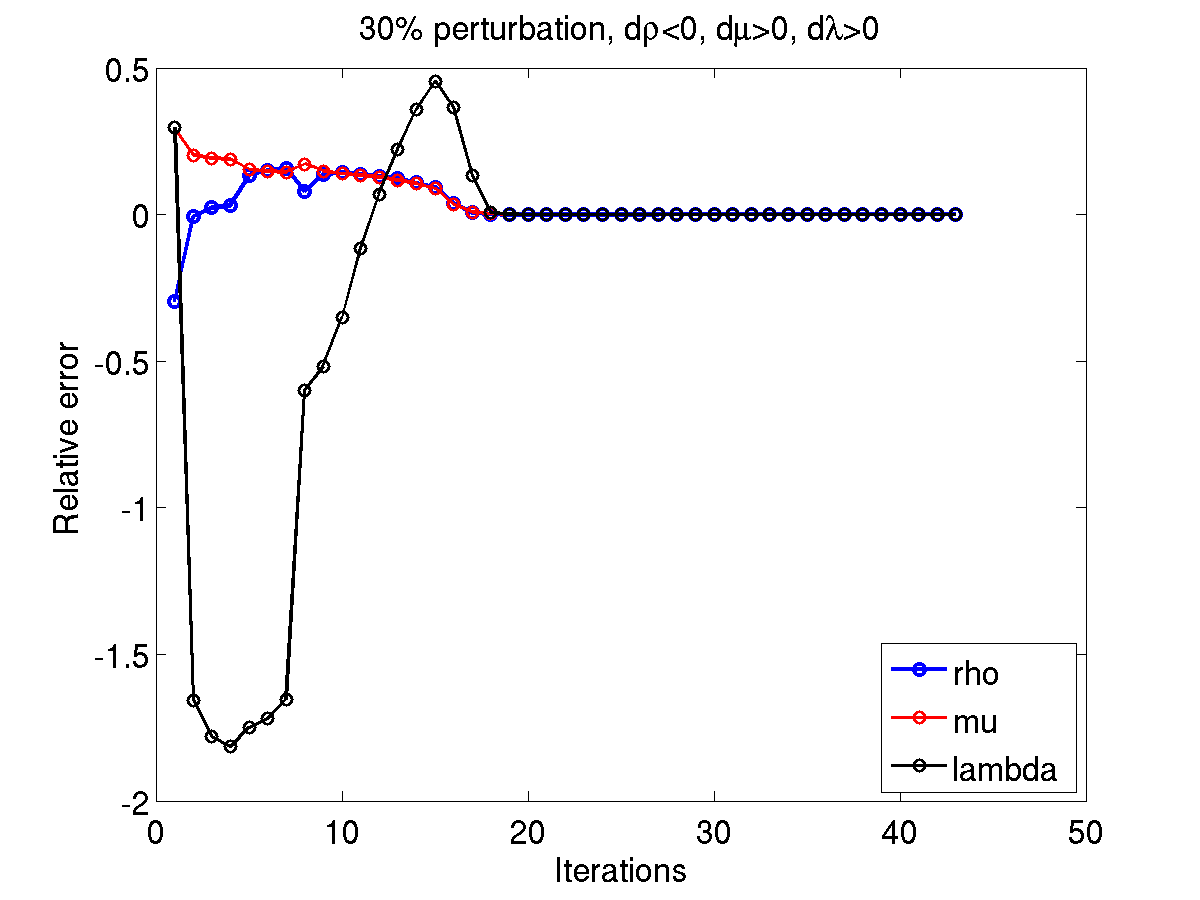
\includegraphics[width=0.45\textwidth]{\figdir/per30mp-m.png}
\caption{Convergence of $\rho$ (blue), $\mu$ (red), and $\lambda$ (black) for 
problems pm30 (left) and mp30 (right).}
\label{fig:per30vars}
\end{center}
\end{figure}
\par
The input file for this example contains the material specification
\begin{verbatim}
block vp=4630.76 vs=2437.56 r=2650
mparcart nx=1 ny=1 nz=1 init=onep-pr10.bin
\end{verbatim}
meaning that the reference material is defined by the block command, and the initial 10 percent perturbation
is read from the file \verb+onep-pr10.bin+. This file was prepared externally to \emph{SW4mopt}, by a Matlab script. 
The minimizing algorithm was specified by the lines
\begin{verbatim}
mrun task=minvert mcheck=on tsoutput=on
lbfgs nvectors=3 maxit=100 tolerance=1e-12 linesearch=on 
\end{verbatim}
in the inputfile.


\section{Material with sinusodial variation, $3\times 3\times 2$ material grid}
This test problem has the same dimensions and source as the problem in the previous subsection. The 
synthetics are computed on a constant material with an added sinusodial variation. The constant material has the 
properties $\rho=2650$, $v_s=2679.5$, and $v_p=5000$, leading to $\mu=1.90\times 10^{10}$ and
$\lambda=2.82\times 10^{10}$.
The amplitude of the sine perturbation is around 10\% in $\rho$, $\mu$ and $\lambda$. 
Figure~\ref{fig:exactm} shows the density on the plane $z=1000$ at the exact minimum. 
\begin{figure}
\begin{center}
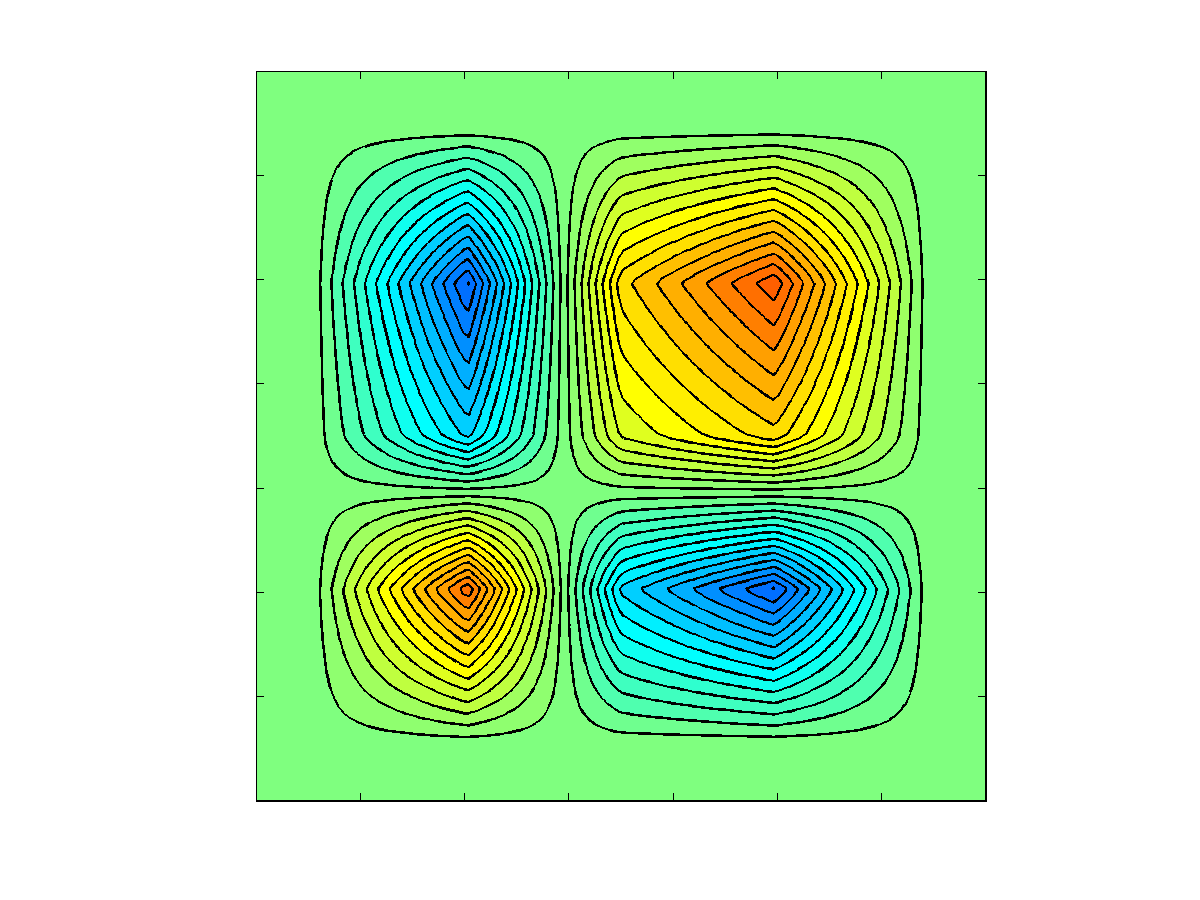
\includegraphics[width=0.7\textwidth]{\figdir/rh-ex.png}\hfil
\caption{Density on the plane $z=1000$ at the exact minimum.}
\label{fig:exactm}
\end{center}
\end{figure}
\par
The inversion algorithm starts from the constant material as initial guess, and iterates to find the
sinusodial material variation. As an illustration of the convergence process, the density 
in the plane $z=1000$, with the same contour levels are plotted in Fig.~\ref{fig:rho-its}.
\begin{figure}
\begin{center}
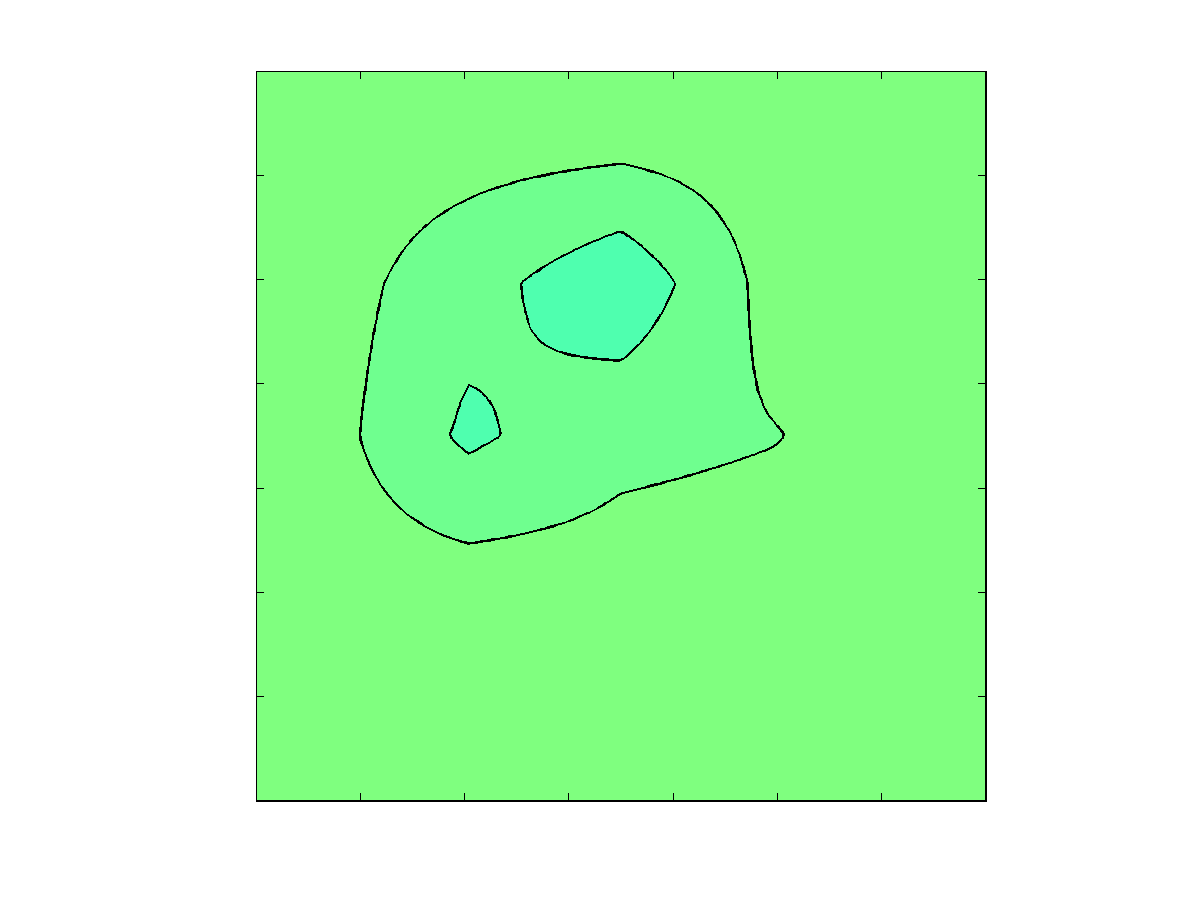
\includegraphics[width=0.33\textwidth]{\figdir/rh-it1.png}\hfil
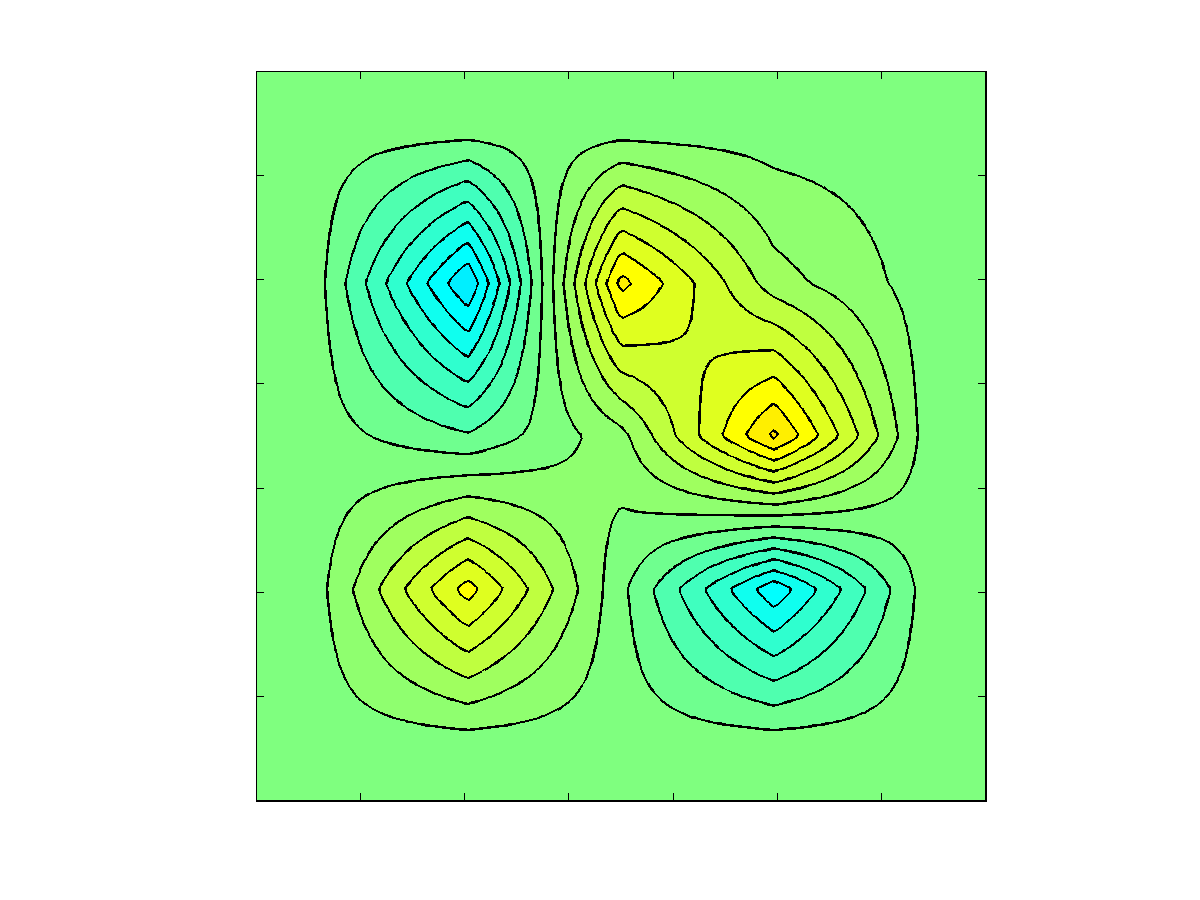
\includegraphics[width=0.33\textwidth]{\figdir/rh-it10.png}\hfil
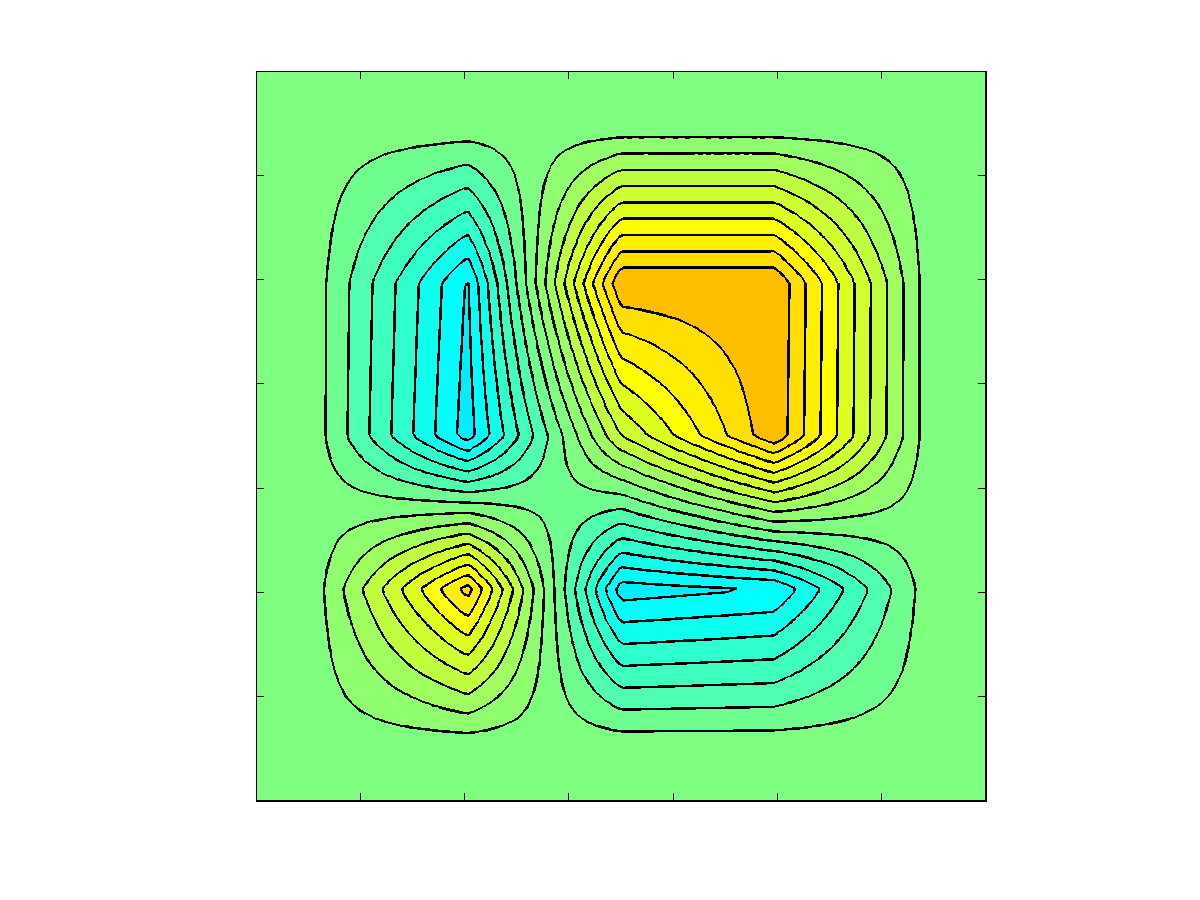
\includegraphics[width=0.33\textwidth]{\figdir/rh-it20.png} \\
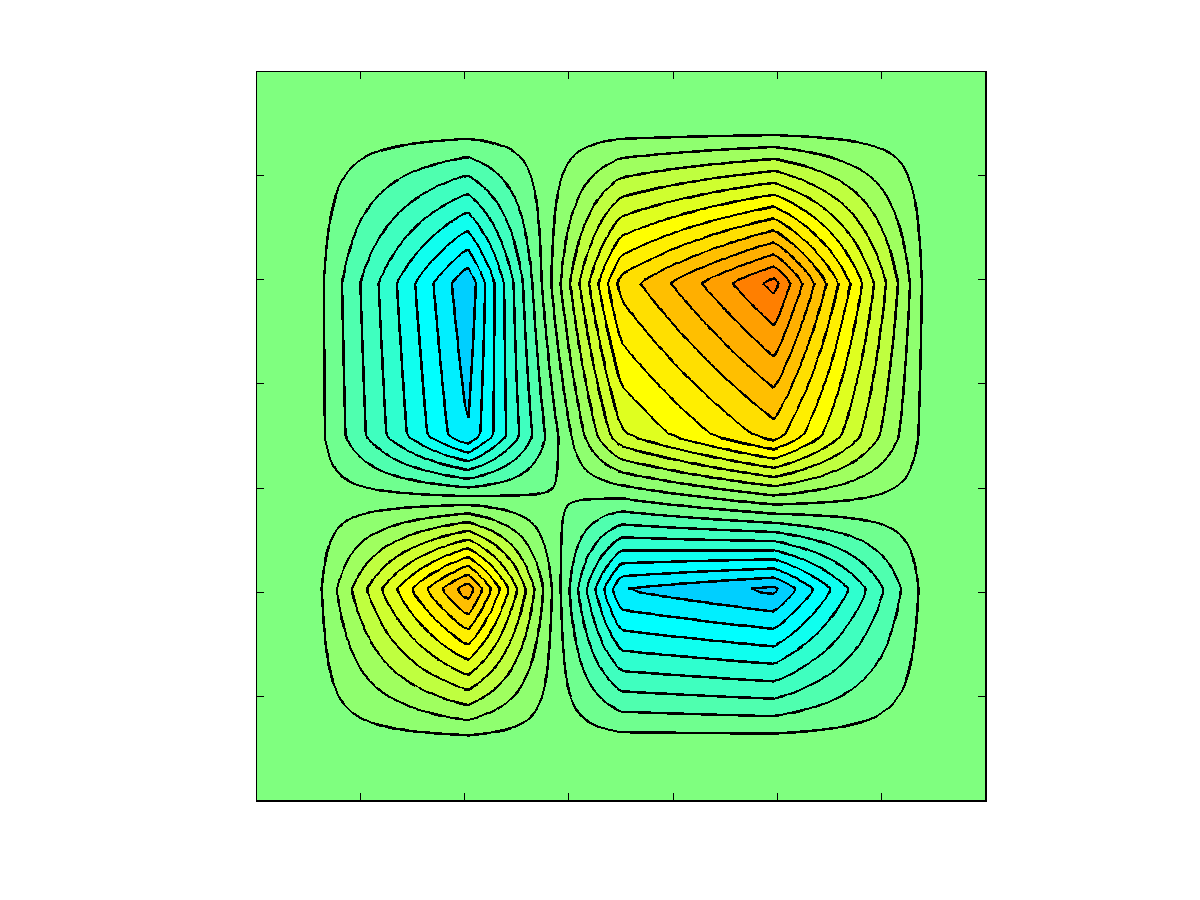
\includegraphics[width=0.33\textwidth]{\figdir/rh-it30.png}\hfil
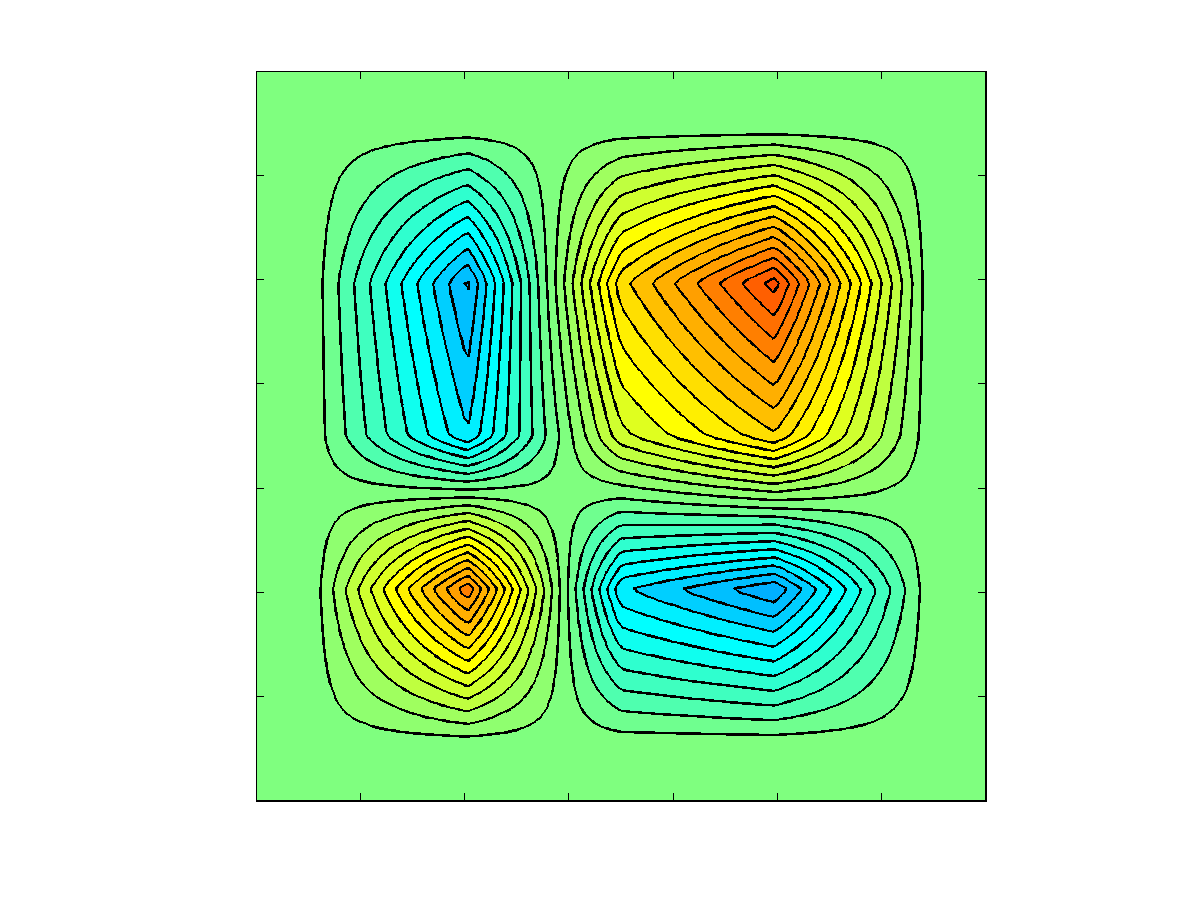
\includegraphics[width=0.33\textwidth]{\figdir/rh-it40.png}\hfil
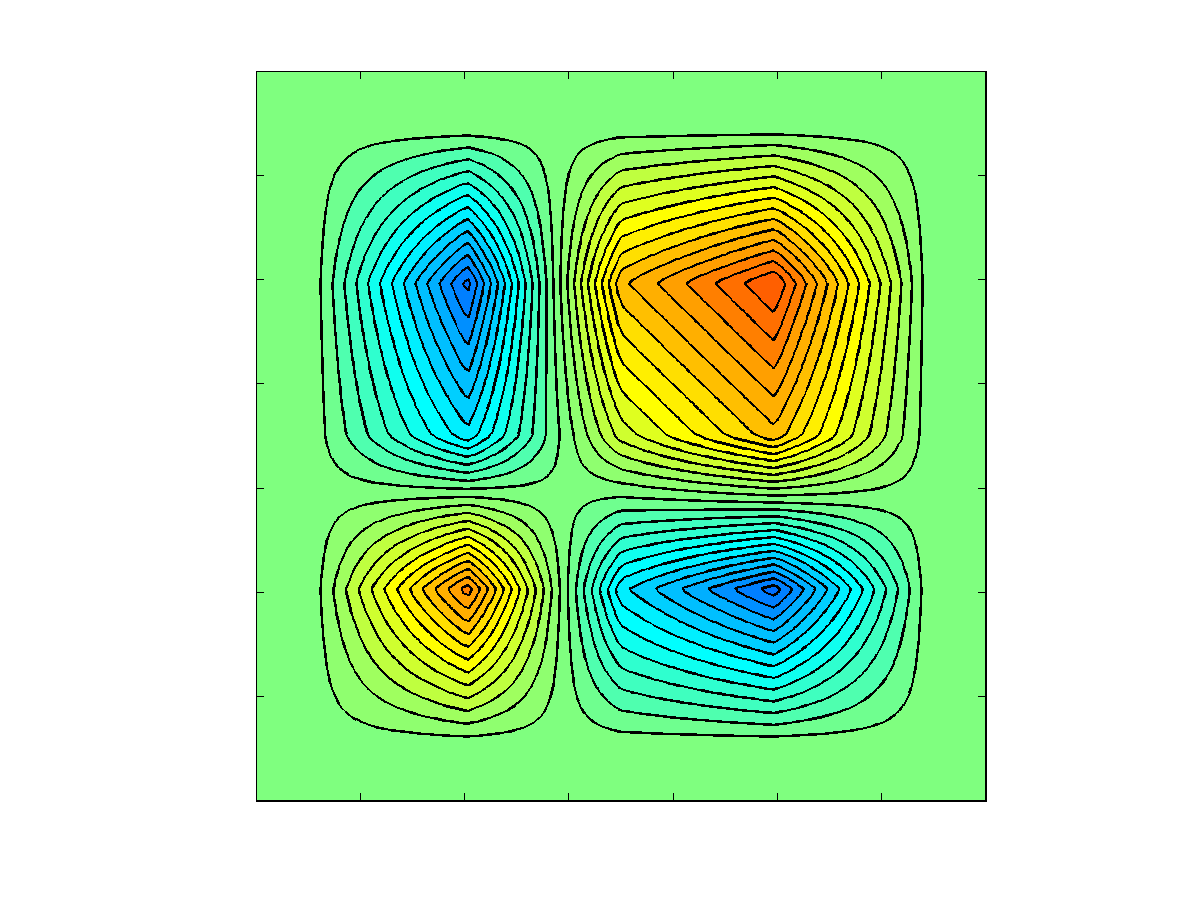
\includegraphics[width=0.33\textwidth]{\figdir/rh-it50.png} \\
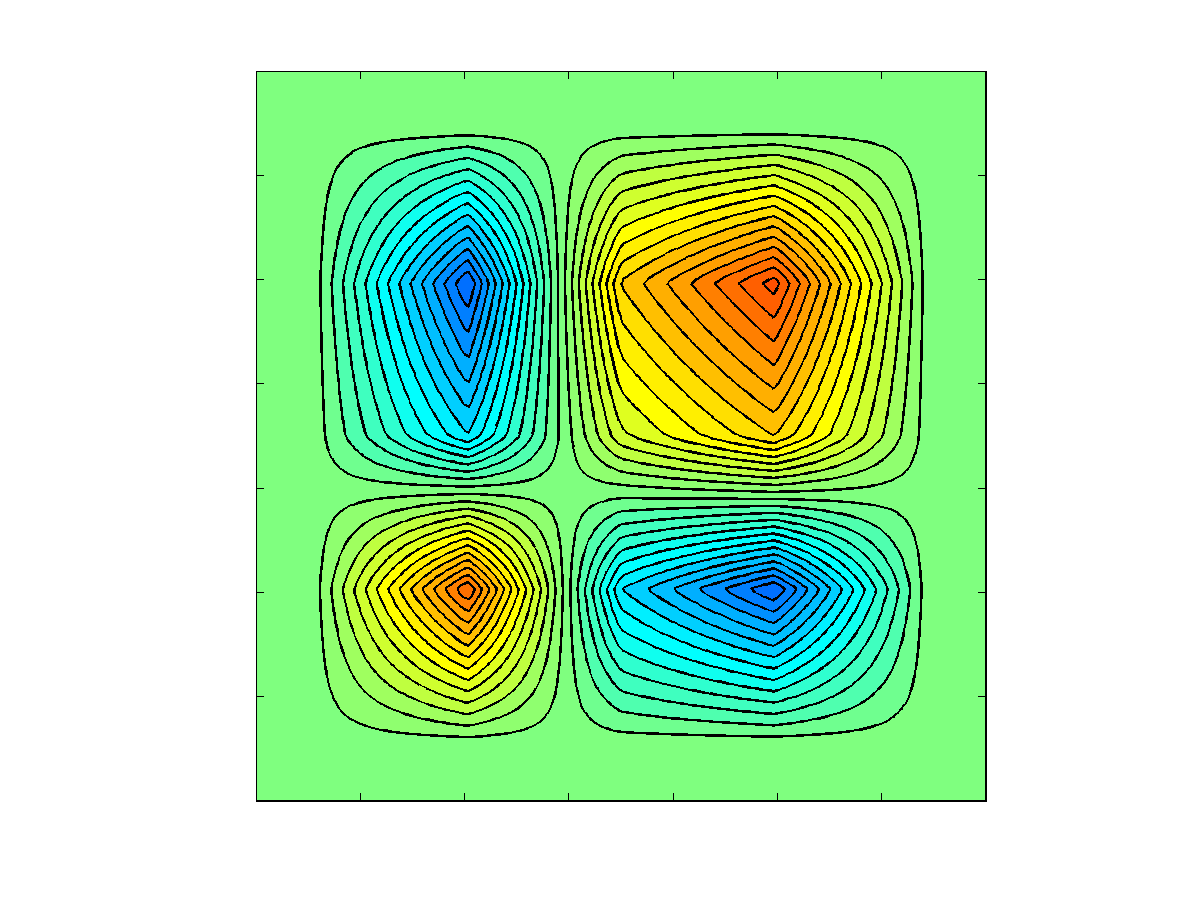
\includegraphics[width=0.33\textwidth]{\figdir/rh-it60.png}\hfil
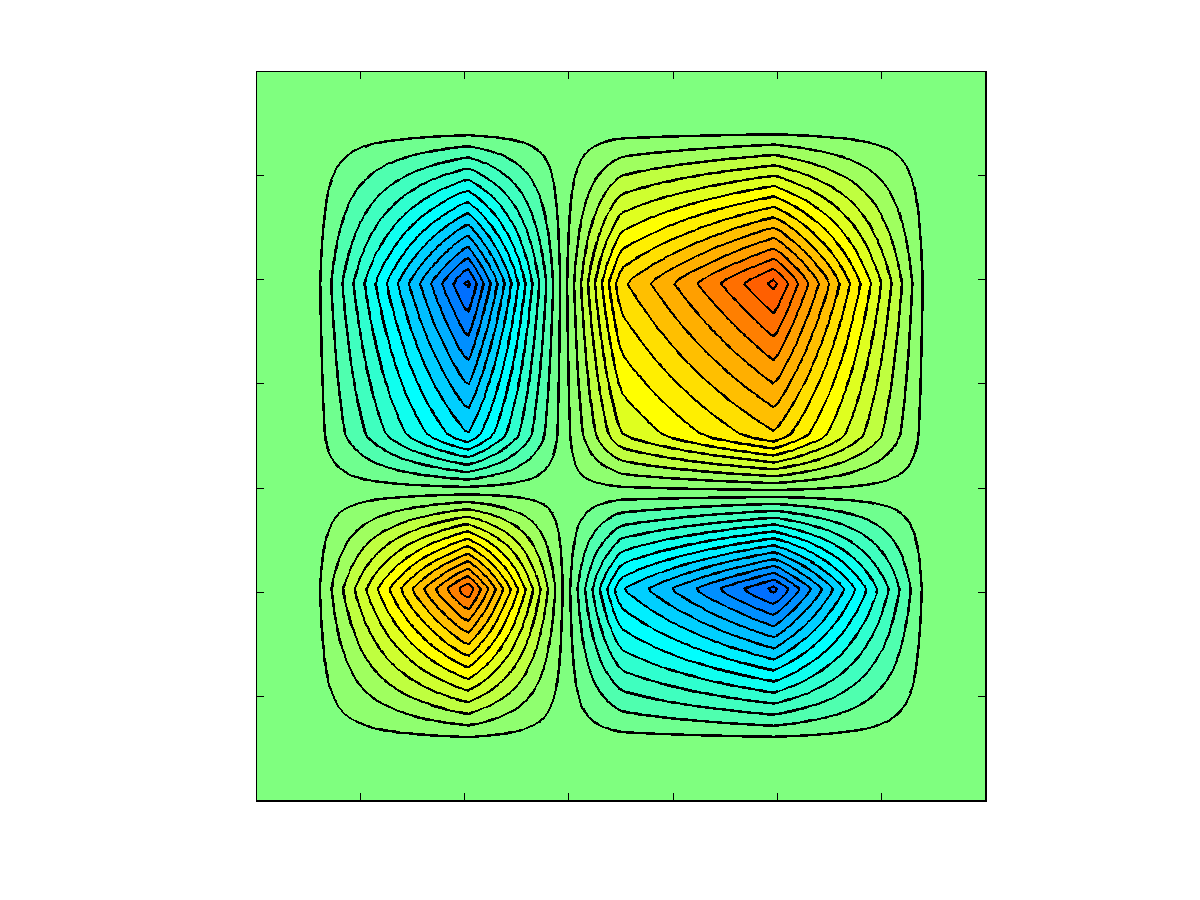
\includegraphics[width=0.33\textwidth]{\figdir/rh-it70.png}\hfil
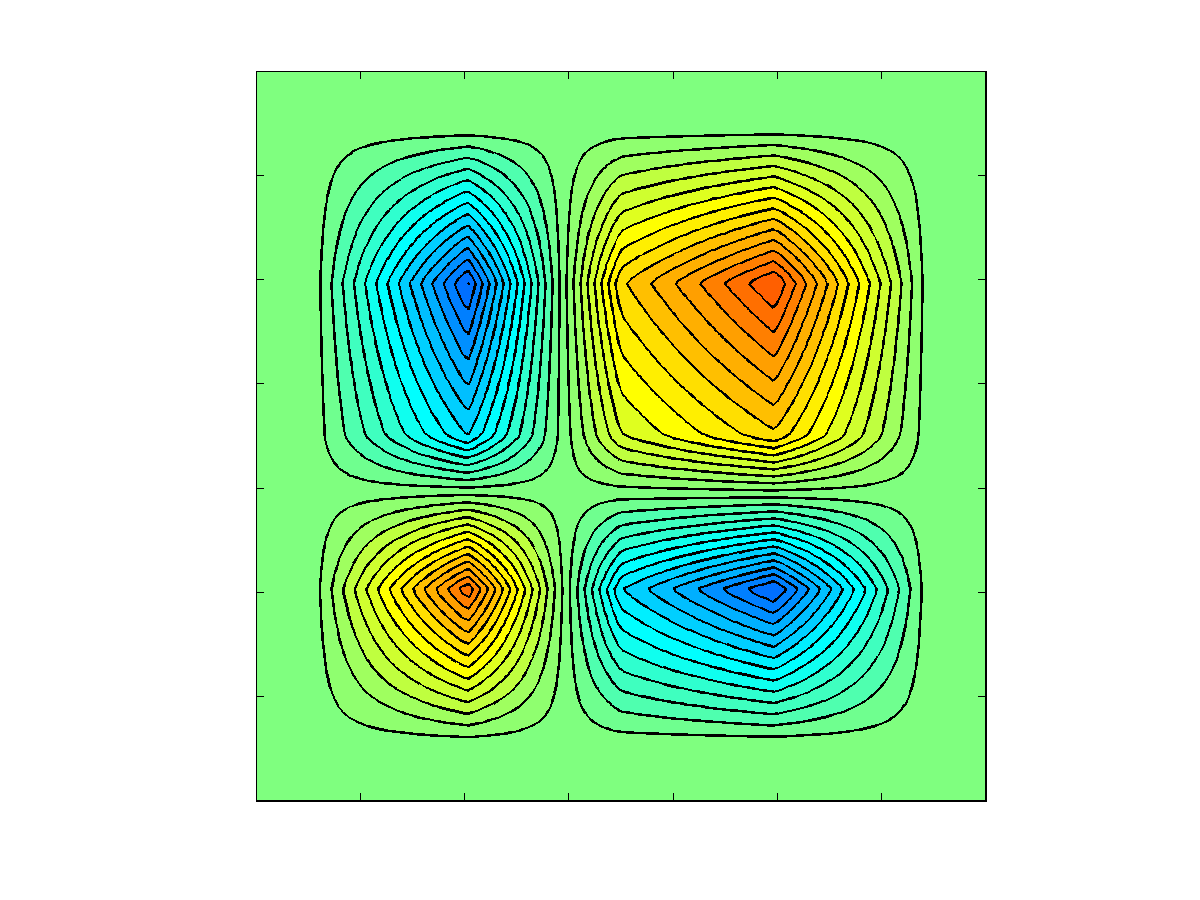
\includegraphics[width=0.33\textwidth]{\figdir/rh-it80.png} \\
\caption{Density on the plane $z=1000$ after 1, 10, 20, 30, 40, 50, 60, 70, and 80 iterations
with the L-BFGS method.}
\label{fig:rho-its}
\end{center}
\end{figure}
\par
Just as in the case with one material grid point, the Lam\'e parameter $\lambda$ shows the largest
variation during the iteration process. The evolution of $\lambda$ is displayed in Fig.~\ref{fig:lambda-its},
showing it out of range of the plotting contour levels after 10, 20, and 40 iterations.
\par
\begin{figure}
\begin{center}
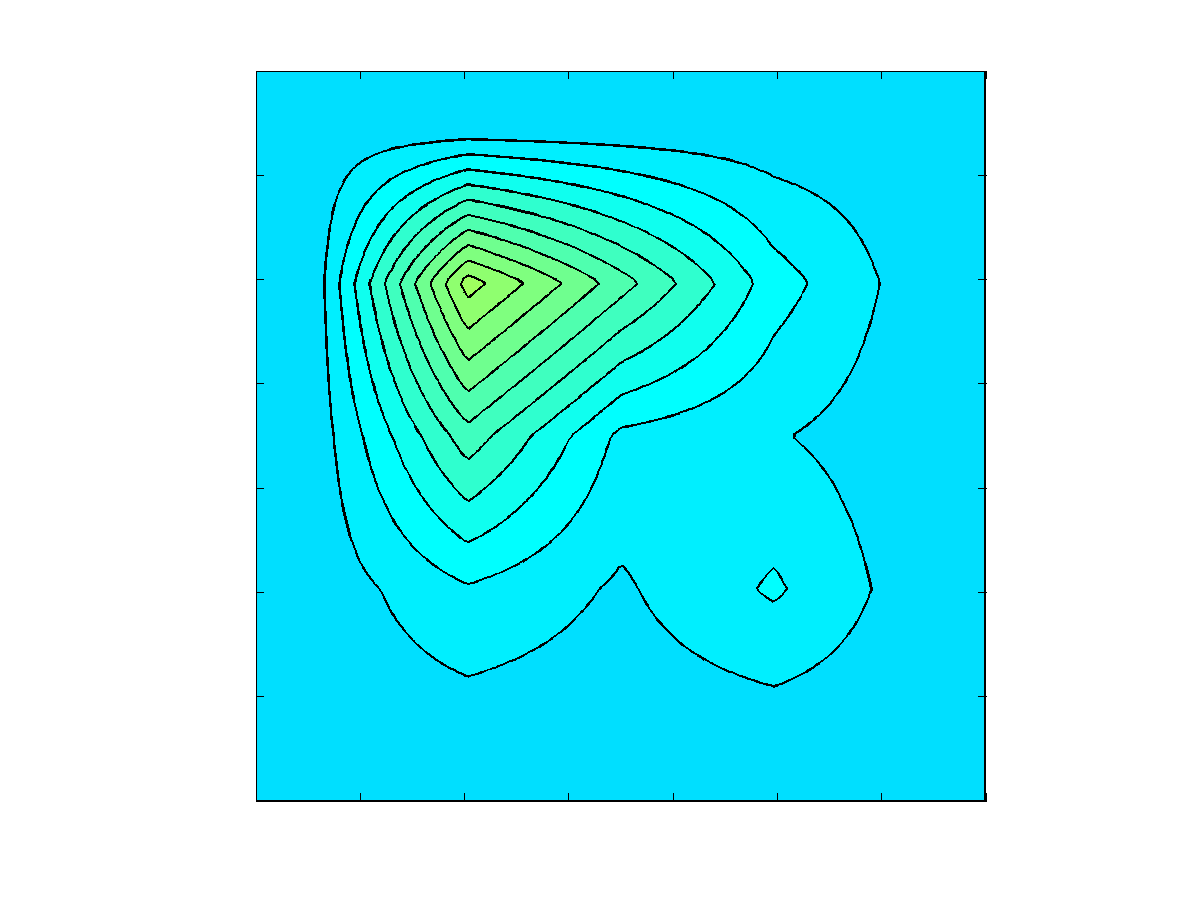
\includegraphics[width=0.33\textwidth]{\figdir/la-it1.png}\hfil
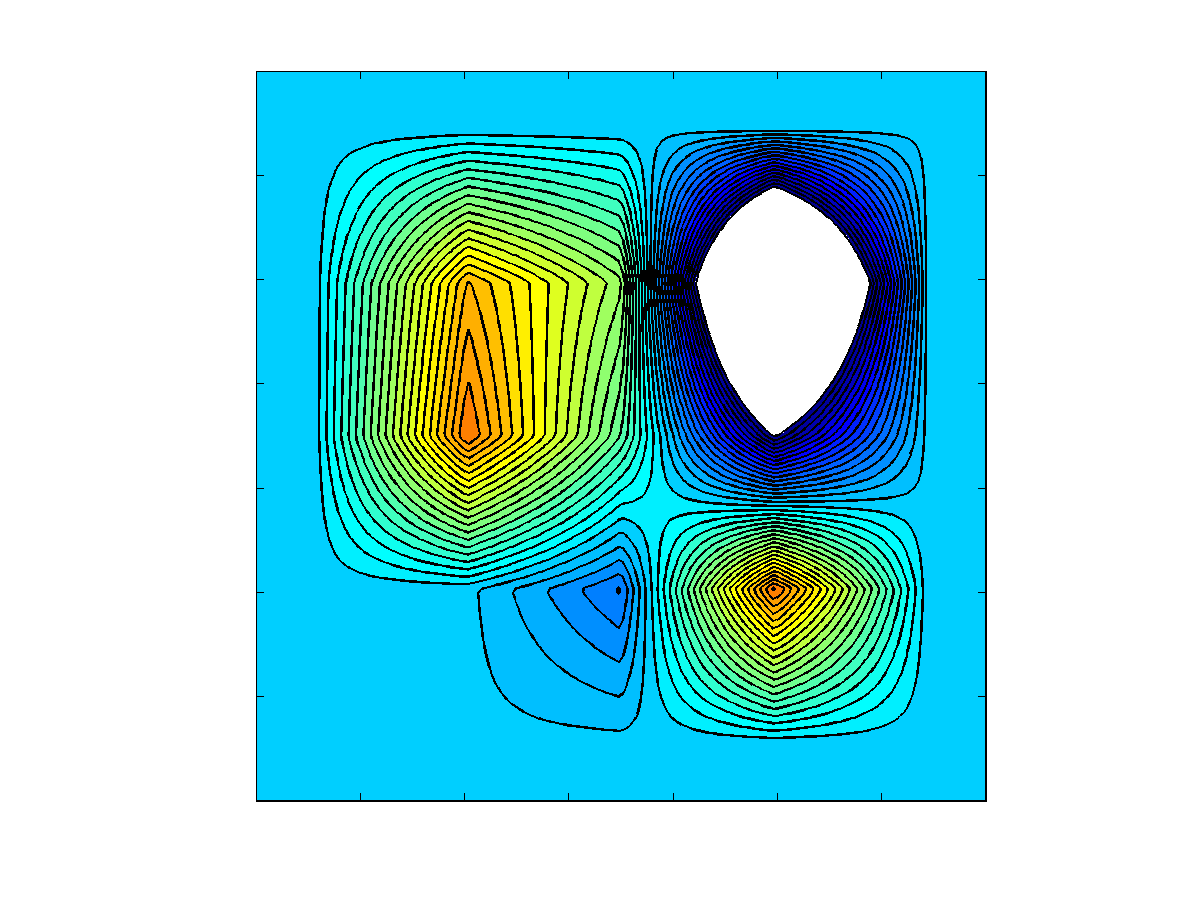
\includegraphics[width=0.33\textwidth]{\figdir/la-it10.png}\hfil
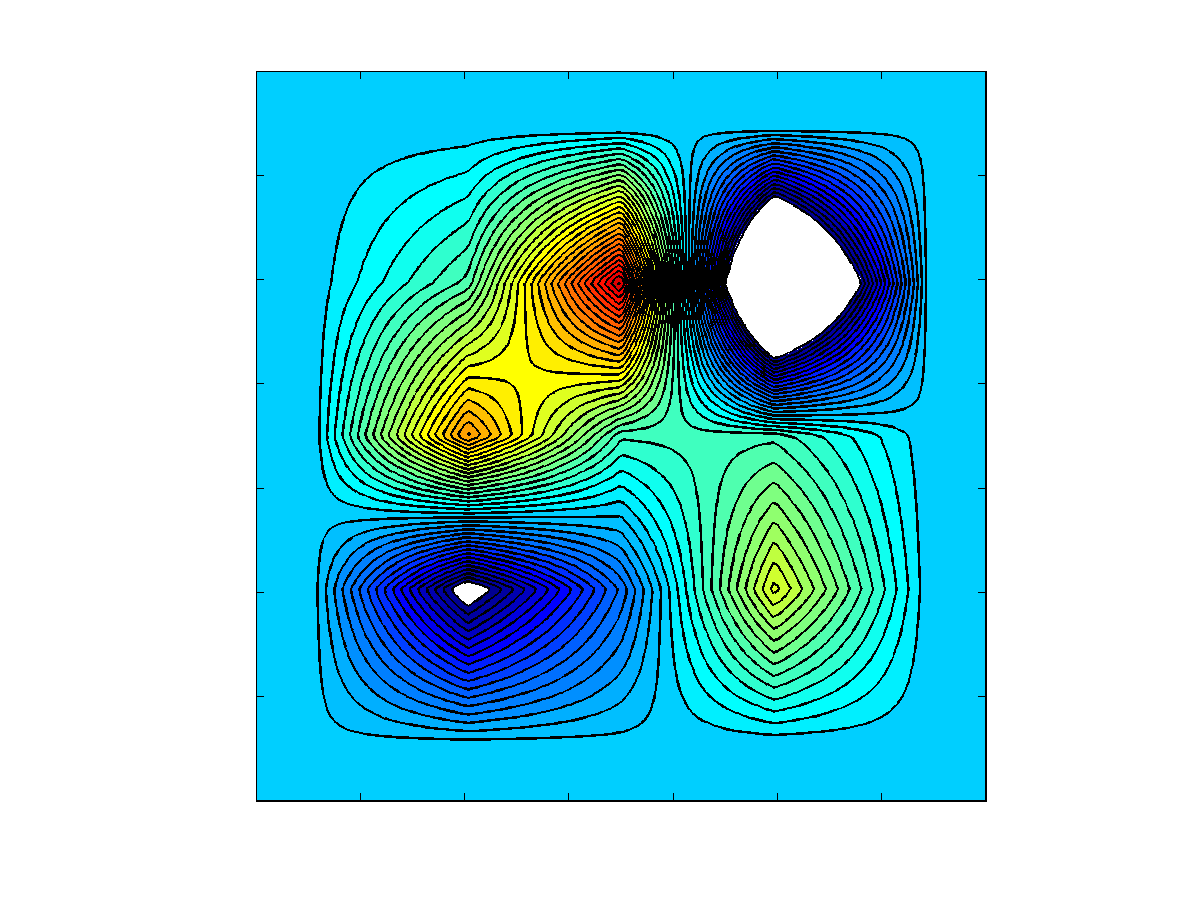
\includegraphics[width=0.33\textwidth]{\figdir/la-it20.png} \\
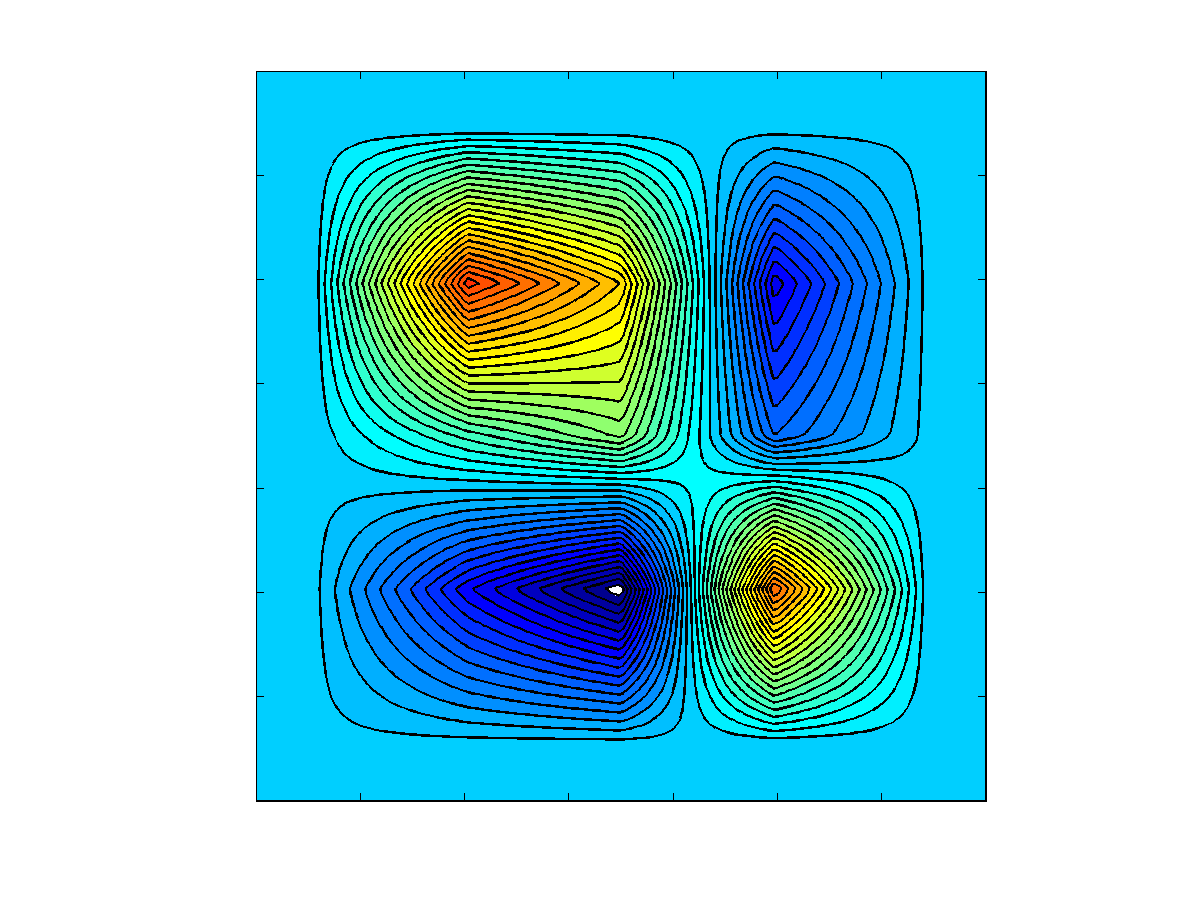
\includegraphics[width=0.33\textwidth]{\figdir/la-it30.png}\hfil
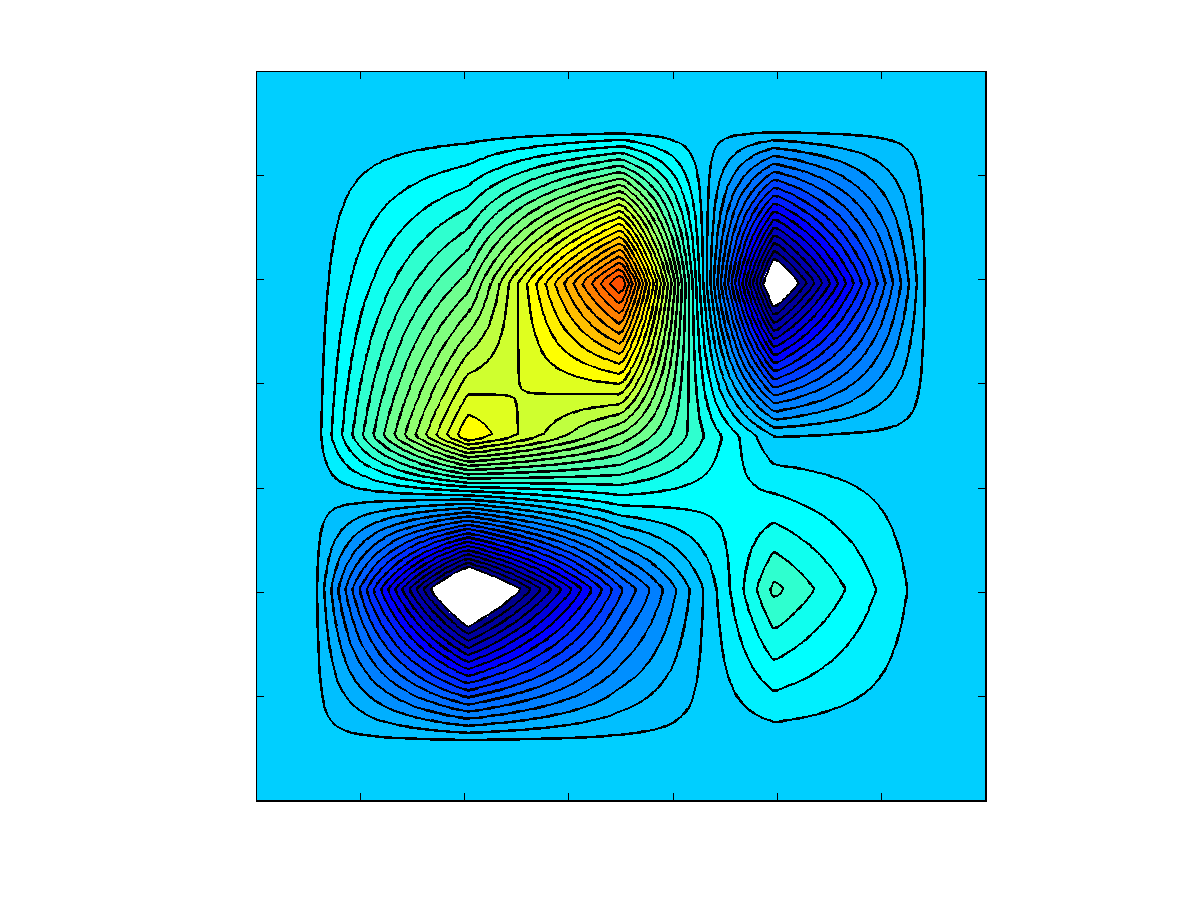
\includegraphics[width=0.33\textwidth]{\figdir/la-it40.png}\hfil
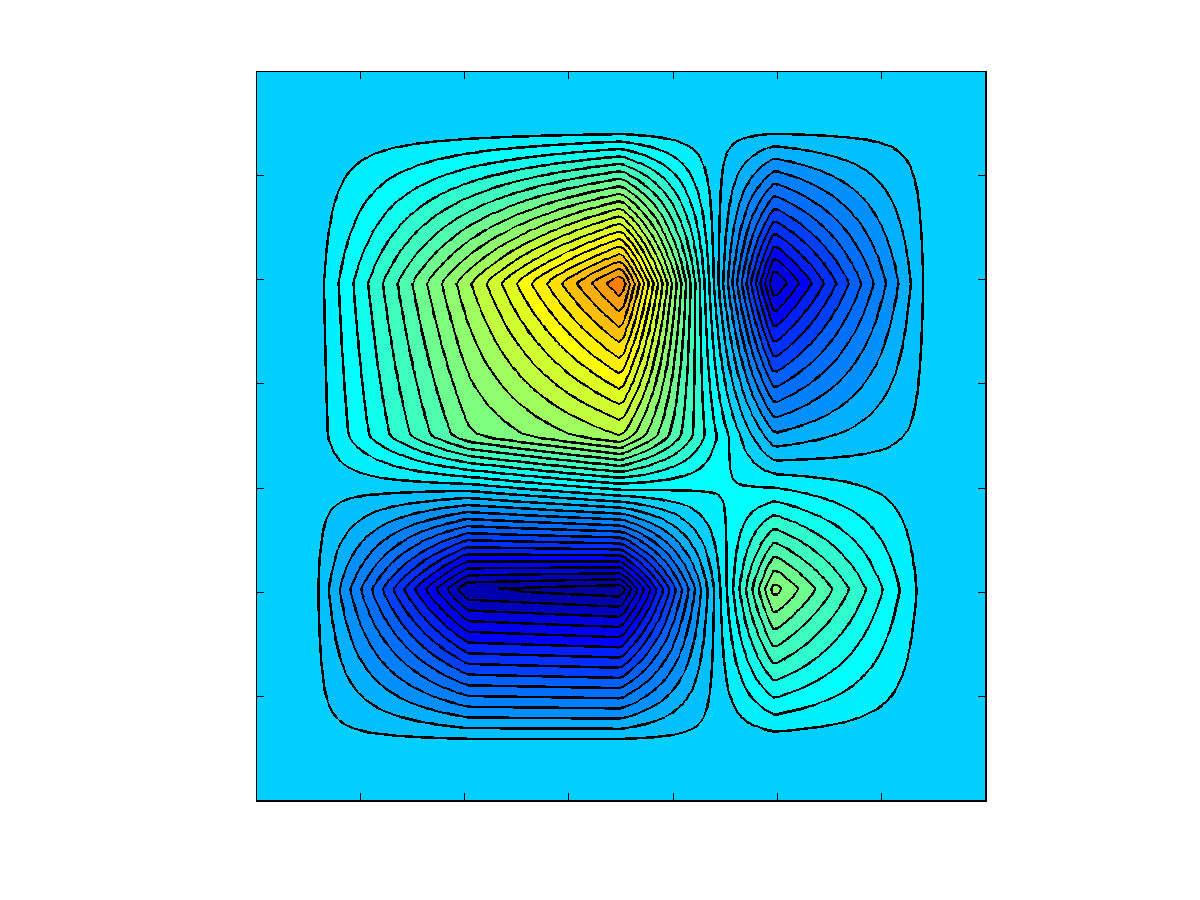
\includegraphics[width=0.33\textwidth]{\figdir/la-it50.png} \\
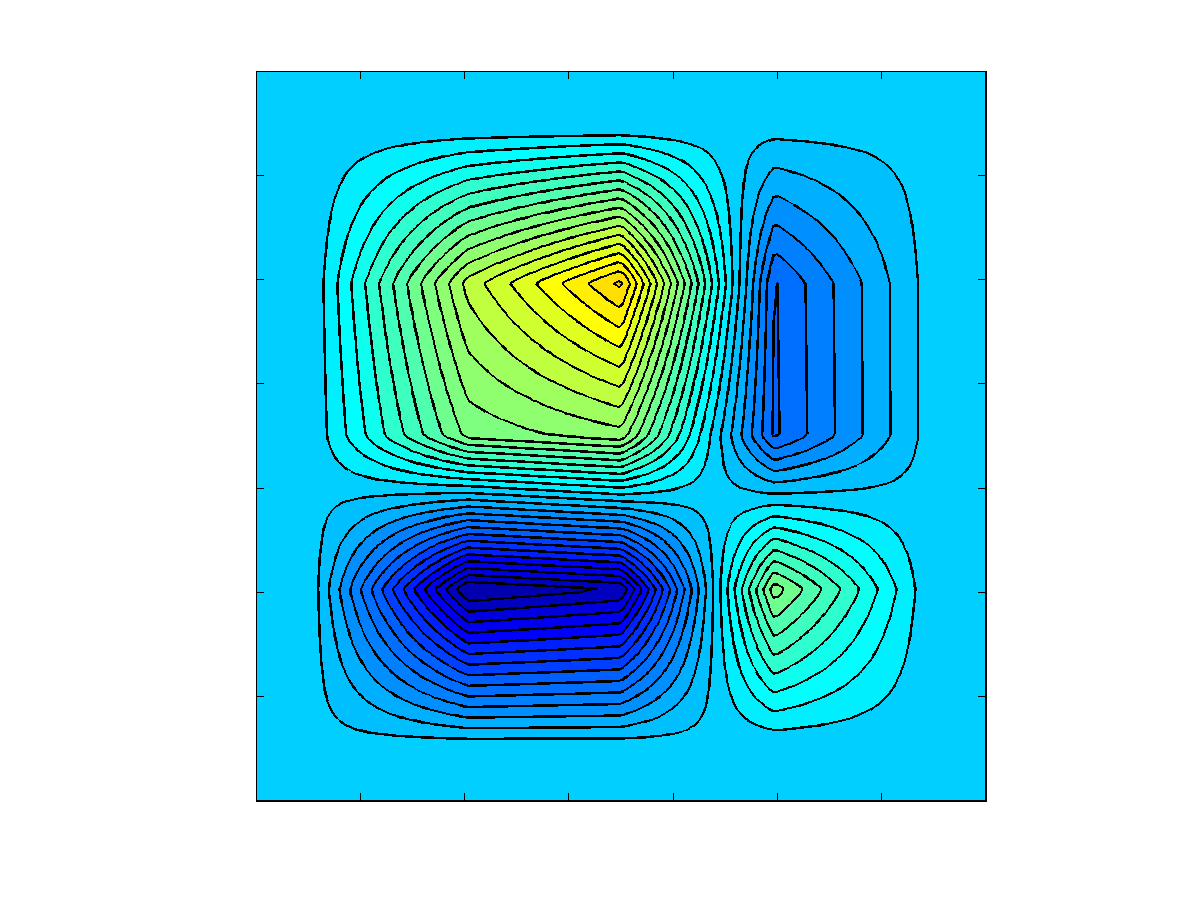
\includegraphics[width=0.33\textwidth]{\figdir/la-it60.png}\hfil
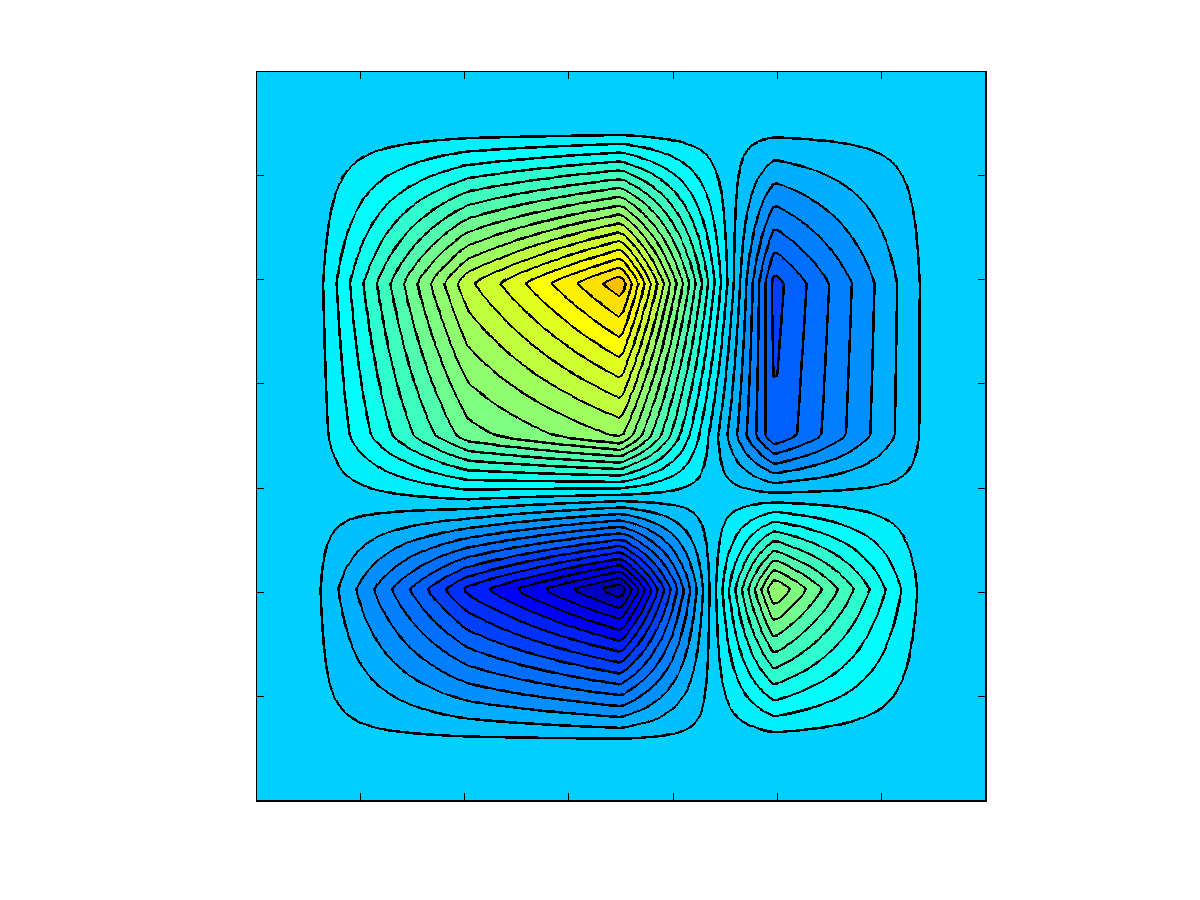
\includegraphics[width=0.33\textwidth]{\figdir/la-it70.png}\hfil
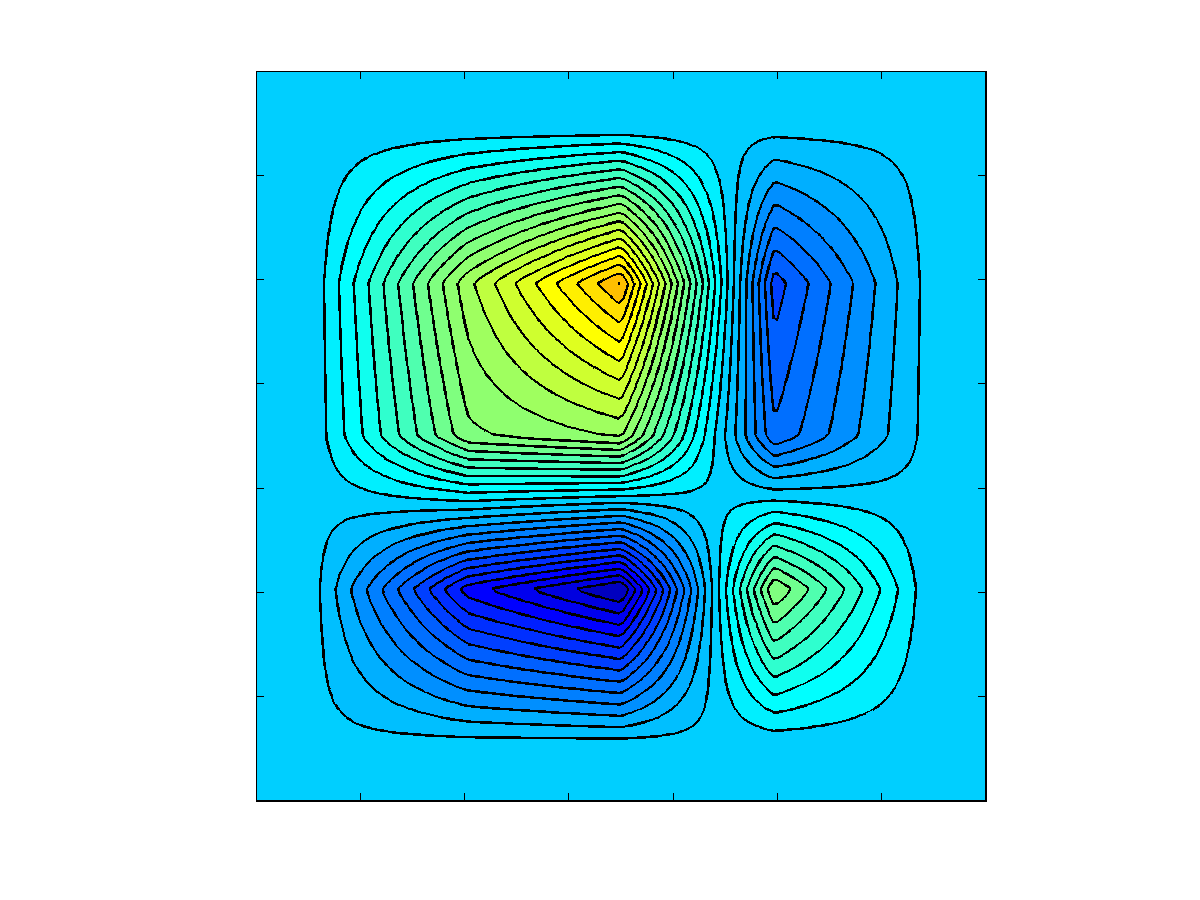
\includegraphics[width=0.33\textwidth]{\figdir/la-it80.png} \\
\caption{Lam\'e parameter $\lambda$ on the plane $z=1000$ after 1, 10, 20, 30, 40, 50, 60, 70, and 80 iterations
with the L-BFGS method.}
\label{fig:lambda-its}
\end{center}
\end{figure}
\par
The convergence in Fig.~\ref{fig:sine-conv}, shows that around 200 iterations are needed to drive down
the misfit to the level of round-off. However, Figs.~\ref{fig:rho-its} and \ref{fig:lambda-its} show that
50--60 iterations give a satisfactory picture of the material, corresponding do a misfit reduction of
4--5 orders of magnitude. 
\begin{figure}
\begin{center}
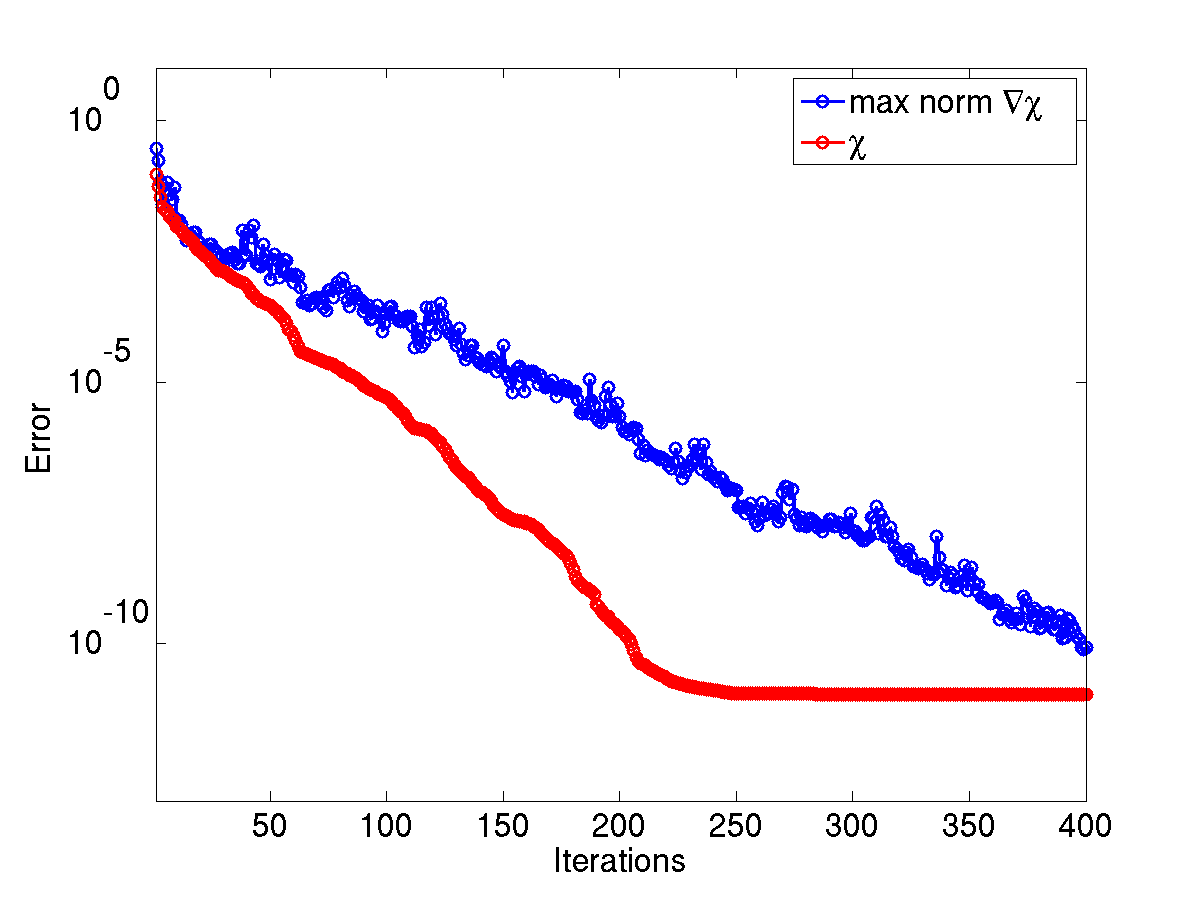
\includegraphics[width=0.7\textwidth]{\figdir/conv-run6.png}\hfil
\caption{Convergence of misfit (red) and maximum norm of the gradient of the misfit (blue) for 
the computation shown in Fig.~\ref{fig:rho-its}.}
\label{fig:sine-conv}
\end{center}
\end{figure}
\par
The input file for this example is given by
\begin{verbatim}
grid h=200 x=35000 y=35000 z=19500
time t=9 utcstart=09/10/2013:23:5:53.000
fileio verbose=1 path=run8 obspath=obs temppath=/tmp/bjorn pfs=1
supergrid gp=13 dc=.015
#
block r=2650 vs=2677.6503357897 vp=4998.11285141419
mparcart nx=3 ny=3 nz=2 init=0
#
mrun task=minvert mcheck=on 
lbfgs nvectors=35 maxit=300 tolerance=1e-12 linesearch=on ihess0=scale-factors
mscalefactors rho=2650 mu=1.19e10 lambda=5.10e11 
#
source x=17500 y=17500 z=2000 Mxy=1 m0=1e18 t0=1.5 freq=4 type=Gaussian
#
developer cfl=1.1
#
observation x=11500 y=11500 z=0 file=sta11
observation x=14500 y=11500 z=0 file=sta21
observation x=17500 y=11500 z=0 file=sta31
 ....
\end{verbatim}
The first four lines set up the domain and discretization size. It uses the same syntax as the forward
solver, \emph{SW4}. The only additional items for the inverse problem are the two new paths,
\verb+obspath+ and \verb+temppath+, given at the \verb+fileio+ command. The \verb+obspath+ is the directory
containing the observed seismograms. These data are read by the solver, nothing is output into \verb+obspath+.
\par
The \verb+temppath+ is a directory where temporary files associated with the outflow boundaries are stored.
In order to reconstruct the forward solution during the backward solve, the forward solution on the outflow
boundaries needs to be saved. Each processor that holds a part of the outflow boundary, writes its own
file to \verb+temppath+. These files can become fairly large, and there can be a lot of them. The read and write
speeds to \verb+temppath+ will have a major effect on the preformance of the inverse solver. 
Preferably, \verb+temppath+ should be a directory on a disk that is local to the computational node. 
On the LC sytems, the directory \verb+/tmp/username+ is usually a good choice, if the files are not too large.
The temporary files are deleted by \emph{SW4mopt} when they are no longer needed, however if the program
crashes, files might be left in \verb+temppath+.
\par
The next two lines, 
\begin{verbatim}
block r=2650 vs=2677.6503357897 vp=4998.11285141419
mparcart nx=3 ny=3 nz=2 init=0
\end{verbatim}
specify the material repesentation and the initial guess material. The computation starts from a zero 
perturbation on the constant reference material described by the \verb+block+ command. The material grid 
has $3\times 3\times 2$ points. 
\par
The L-BFGS method is specified by 
\begin{verbatim}
lbfgs nvectors=35 maxit=300 tolerance=1e-12 linesearch=on ihess0=scale-factors
\end{verbatim}
A maximum of 300 iterations are taken, using 35 L-BFGS vectors. The initial inverse Hessian will be
computed from the scale factors. These are specified on the \verb+mscalefactors+ line below. The
scale factors are also used to compute the step length in the minimization algorithm.
\par
The source is given below the \verb+mscalefactors+ line. The source is specified with exactly the 
same syntax as in the forward solver. Below the \verb+source+ command, the CFL-number is set to 1.1. 
In \emph{SW4mopt}, the maximum allowed CFL-number is hard coded to 1.3. By computing with a somewhat lower 
CFL-number, we allow the material wave speeds to increase by (1.3-1.1)/1.1 = 18\% during the minimization. 
\emph{SW4mopt} never changes the initially computed time step. However, the line search algorithm restricts
the step size of the minimizer so that the maximum CFL-limit 1.3 is always respected. 
If the material makes the CFL-number getting too close to 1.3, the minimization step length will go 
to zero, and the minimizer fails. In that case, the computation has to be restarted with a 
smaller CFL-number. 
\par
The synthetic seismograms were prepared by the forward solver, run in the perturbed material. The
seismograms are output in USGS-format, on files \verb+sta11.txt+, \verb+sta21.txt+, etc. up
to \verb+sta55.txt+. The synthetics are read into \emph{SW4mopt} by the commands
\begin{verbatim}
observation x=11500 y=11500 z=0 file=sta11
observation x=14500 y=11500 z=0 file=sta21
observation x=17500 y=11500 z=0 file=sta31
....
\end{verbatim}
etc. for all 25 stations. The synthetics were time stamped by the forward solver. The UTC time is
registered in the header of the output time series on USGS-format. In this example, the UTC time
was September 10th 2013 at 23:5:53. It is important that we specify the same start time for the 
inverse solver. This is done by the command
\begin{verbatim}
time t=9 utcstart=09/10/2013:23:5:53.000
\end{verbatim}
in the input file.

%-----------------------------------------------------------------------
\chapter{Keywords in the input file}\label{chap:keywords}
The syntax of the input file is the same as in the forward solver, \emph{SW4}. The input
file consists of a number of lines with statements
\begin{verbatim}
command1 parameter1=value1 parameter2=value2 ... parameterN=valueN
# comments are disregarded
command2 parameter1=value1 parameter2=value2 ... parameterM=valueM
...
\end{verbatim}
Each command starts at the beginning of the line and ends at the end of the same line. Blank and
comment lines are disregarded. A comment is a line starting with a \# character. The order of the
parameters within each command makes no difference. 

Parameter values are either integers (-2,0,5,...), real numbers (20.5, -0.05, 3.4e4), or strings
(earthquake, my-favorite-simulation). Note that there must be no spaces around the = signs and
strings are given without quotation marks and must not contain spaces. 

A breif description of all commands is given in the following sections. The commands marked as
[required] must be present in all \emph{SW4mopt} input files, while those marked as [optional] are just
that. 

\section{Material optimizer}

\subsection{The mrun command}\label{sec:mrun}
\begin{flushleft}\bf
Syntax:\\
\tt
mrun task=... mcheck=... tsoutput=... 
\\
\bf Required parameters:\\
\rm
None
\end{flushleft}
The \verb+mrun+ command specifies which task to perform. The possible tasks are
given in the table below. 
\begin{center}
\begin{tabular}{|l|p{8cm}|l|l|l|} \hline
\multicolumn{2}{|c|}{\bf possible values of the task option}\\ \hline
{\bf Option} & {\bf Description}           \\ \hline 
\hline
minvert     & Perform material inversion (default) \\ \hline
gradtest    & Test gradient computation vs.~a numerical derivative \\ \hline
hesstest    & Compute the Hessian numerically  \\ \hline
func1d      & Compute and output a one dimensional cut of the misfit \\ \hline
func2d      & Compute and output a two dimensional surface of the misfit \\ \hline
forward     & Run one forward solve and exit. \\ \hline
minvert+src11& Perform material and source inversion, 11 parameter source. \\ \hline
minvert+src10& Perform material and source inversion, 10 parameter source. \\ \hline
minvert+src9& Perform material and source inversion, 9 parameter source. \\ \hline
minvert+src6& Perform material and source inversion, 6 parameter source. \\ \hline
\end{tabular}
\end{center}
Further specification of the {\tt func1d}, {\tt func2d} tasks, e.g., which parameter to
vary, can be done with the \verb+msurf+ command. The generated cut/surface is output on
a file named {\tt fsurf.bin}, the format of which is described in Section~\ref{}.
\par
The intended use of \verb+task=forward+ is to
generate synthetic seismograms for testing the material inversion. \par
\verb+mcheck=on+ tells the optimizer to check the computed material for reasonableness, e.g.,
that the density and $\mu$ are positive, after each iteration. \verb+tsoutput=on+ causes
the time series (synthetic seismograms) to be output after each iteration.
\verb+mcheck+ and \verb+tsoutput+ are only effective when the task is \verb+minvert+.
\begin{center}
\begin{tabular}{|l|p{6cm}|l|l|l|} \hline
\multicolumn{4}{|c|}{\bf mrun command parameters}\\ \hline
{\bf Option} & {\bf Description}          & {\bf Type} & {\bf Default} \\ \hline 
\hline
task    & task to perform                 & string & minvert \\ \hline
mcheck  & material checking (on or off)   & string & off \\ \hline
tsoutput & output time series (on or off) & string & off \\ \hline
\end{tabular}
\end{center}

Currently, mcheck only outputs diagnostic messages, no attempt to correct the material if
it is out of range is made.

\subsection{The lbfgs command}\label{sec:lbfgs}
\begin{flushleft}\bf
Syntax:\\
\tt
lbfgs nvectors=... ihess0=... maxit=... tolerance=... linesearch=...
\\
\bf Required parameters:\\
\rm
None
\end{flushleft}
Configure the L-BFGS method for minimizing the misfit. L-BFGS will iterate until \verb+maxit+ iterations
are reached, or until the maximum norm of the scaled gradient of the misfit is less than \verb+tolerance+. 
\par
The option {\tt linesearch=off} switches off the line search step of L-BFGS. This is usually not stable.
The default {\tt linesearch=on} switches on a standard line search algoritm. However, L-BFGS is only guaranteed to
be stable if the so called Wolfe condition is satisfied. The option {\tt linesearch=wolfe} switches on
the line search with additional logic to satisfy the Wolfe condition. Line search with the Wolfe condition 
is computationally expensive, since the gradient of the misfit has to be evaluated at least once. Therefore,
it is advisable to try the standard line search first, we have found it to work satisfactory in many cases.
\par
L-BFGS builds and approximation of the inverse Hessian, represented by \verb+nvectors+ vectors, which can
be thought of as a rank-\verb+nvectors+ approximation. The convergence rate is usually better for larger 
values of \verb+nvectors+. The method requires an initial guess for the inverse Hessian. The option
{\tt ihess0=scale-factors} uses an initial guess based on the scale factors of the problem, while
{\tt ihess0=gamma} uses an initial guess by an estimate of the size of the Hessian along the search 
directions, given by formula (7.20) in \cite{Nocedal-Wright}.

\begin{center}
\begin{tabular}{|l|p{7cm}|l|l|l|} \hline
\multicolumn{4}{|c|}{\bf lbfgs command parameters}\\ \hline
{\bf Option} & {\bf Description}          & {\bf Type} & {\bf Default} \\ \hline 
\hline
nvectors   & Number of l-bfgs vectors to keep & int   & 10 \\ \hline
ihess0     & Initial guess for inverse Hessian & string & gamma \\ \hline
maxit      & Maximum number of iterations  & int & 10 \\ \hline
tolerance  & Termination criterion for gradient  & float & $10^{-12}$ \\ \hline
linesearch  & Line search method (on, off, or wolfe)  & string & on \\ \hline
\end{tabular}
\end{center}

\subsection{The nlcg command}\label{sec:nlcg}
\begin{flushleft}\bf
Syntax:\\
\tt
nlcg maxit=... tolerance=... linesearch=... subtype=... maxsubit=...
\\
\bf Required parameters:\\
\rm
None
\end{flushleft}
Configure the non-linear conjugate gradient (NLCG) method for minimizing the misfit. NLCG will iterate 
until \verb+maxit+ restarts are reached, or until the maximum norm of the scaled gradient of the 
misfit is less than \verb+tolerance+. CG methods are usually restarted every $n$th iteration, 
where $n$ is the number of unknowns. The behavior of the iterations is controlled by the two 
parameters \verb+maxit+ and \verb+maxsubit+. \verb+maxit+ gives the maximum number of restarts, 
and \verb+maxsubit+ is the number of iterations between the restarts. By default \verb+maxsubit+ 
is set to $n$. 
\par
The option {\tt linesearch=off} switches off the line search step in NLCG. 
The default {\tt linesearch=on} switches on a standard line search algoritm. 
The initial step size is computed by approximating the minimization functional by
a quadratic surface.
\par
The \verb+subtype+ option makes it possible to specify the Fletcher-Reeves or the
Polak-Ribi\`ere variants of the NLCG. The Polak-Ribi\`ere algorithm forces a restart
more often than Fletcher-Reeves. With {\tt subtype=polak-ribiere}, \verb+maxit+ needs to 
be set large enough to allow for the additional restarts. 

\begin{center}
\begin{tabular}{|l|p{6cm}|l|l|l|} \hline
\multicolumn{4}{|c|}{\bf nlcg command parameters}\\ \hline
{\bf Option} & {\bf Description}          & {\bf Type} & {\bf Default} \\ \hline 
\hline
maxit       & Maximum number of iterations        & int & 10 \\ \hline
tolerance   & Termination criterion for gradient  & float & $10^{-12}$ \\ \hline
linesearch  & Line search method (on or off)  & string & on \\ \hline
subtype     & fletcher-reeves or polak-ribiere & string  & polak-ribiere \\ \hline
maxsubit    & Number of subiterations in CG & int & \# unknowns \\ \hline
\end{tabular}
\end{center}

\subsection{The mscalefactors command}\label{sec:mscalefactors}
\begin{flushleft}\bf
Syntax:\\
\tt
mscalefactors rho=... mu=... lambda=... file=... misfit=...
\\
\bf Required parameters:\\
\rm
None
\end{flushleft}
Introducing scale factors will improve the convergence rate of the minmizer, by reducing the condition number of 
the Hessian of the misfit. For quadratic problems, the scale factors form a diagonal pre-conditioning
matrix. There is one scale factor for each unknown. Ideally, the scale factor for the $i$th unknown, $x_i$, 
should be $1/\sqrt{H_{ii}}$, where $H_{ii}$ is the $i$th diagonal element of the Hessian. 
The \verb+file=+ option specifies a file name, from which the scale factors are read. The number of scale
factors on the file should be equal to the number unknown parameters. The format of the file is described
in Section~\ref{}.
\par
If the Hessian is not known, an alternative is to set the scale factors to reference sizes of the parameters.
If the material parameterization is made such that each parameter is identifiable with one of the material
properties, $\rho$, $\mu$, or $\lambda$, the options \verb+rho=+, \verb+mu=+, and \verb+lambda=+  can be
used to specify three different scales. These scale factors are used throughout for all unknowns of 
the respective type.
\par
The \verb+misfit=+ is a factor that modifies the input scale factors. It is based on the observation that
the scale of $1/\sqrt{H_{ii}}$, with $H=\partial^2f/(\partial x_i^2)$, is actually $x_r/\sqrt{f_r}$, where
$x_r$ is the scale of the unknown $x_i$, and $f_r$ is the scale of the objective function. All input
scale factors will be divided by the square root of the value of the \verb+misfit+ parameter.
The condition number of the Hessian is not affected by multiplying all factors by a constant, 
but the multiplier will affect the maximum step length, and is currently needed to sometimes reduce the 
allowed step size. This is a temporary measure that should be removed, once the line search algorithm
has been improved.

\begin{center}
\begin{tabular}{|l|p{6cm}|l|l|l|} \hline
\multicolumn{4}{|c|}{\bf mscalefactors command parameters}\\ \hline
{\bf Option} & {\bf Description}          & {\bf Type} & {\bf Default} \\ \hline 
\hline
rho      & Density scale factor                & float & 1 \\ \hline
mu       & Scale of Lam\'e parameter $\mu$     & float & 1 \\ \hline
lambda   & Scale of Lam\'e parameter $\lambda$ & float & 1  \\ \hline
file     & Name of file containing scale factors  & string  & None \\ \hline
misfit & Multiplier for scale factors & float & 1 \\ \hline
\end{tabular}
\end{center}

\subsection{The mfsurf command}\label{sec:mfsurf}
\begin{flushleft}\bf
Syntax:\\
\tt
mfsurf var=... i=... j=... k=... pmin=... pmax=... npts=... var2=... i2=... j2=... k2=... pmin2=... pmax2=... npts2=...
\\
\bf Required parameters:\\
\rm
None
\end{flushleft}
The command \verb+mfsurf+ controls the selections for {\tt mrun task=func1d} and {\tt mrun task=func2d}.
The command assumes that the material parameters can be interpreted as values of
$\rho$, $\mu$, or $\lambda$ on a logically rectangular grid, for example, when using material
parameterization by the \verb+mparcart+ command.\par
\verb+var=+, \verb+i=+, \verb+j=+, \verb+k=+ specify one parameter. For example the density at the
point with index $(3,2,4)$ in the coarse material grid defined by \verb+mparcart+, is selected by
\begin{verbatim}
mfsurf var=rho i=3 j=2 k=4
\end{verbatim}
The command 
\begin{verbatim}
mfsurf var=rho i=3 j=2 k=4 npts=30 pmin=-250 pmax=250
\end{verbatim}
specifies the misfit as function of this parameter on the interval [-250,250], discretized by 30 points.
To compute and save the specified function on a file, run \emph{SW4mopt} with \verb+mrun task=func1d+.
\par
The second set of input variables, \verb+var2=+, \verb+i2=+, etc. are used for the second dimension when
a two dimensional misfit surface is specified with \verb+mrun task=func2d+.
\begin{center}
\begin{tabular}{|l|p{6cm}|l|l|l|} \hline
\multicolumn{4}{|c|}{\bf mfsurf command parameters}\\ \hline
{\bf Option} & {\bf Description}          & {\bf Type} & {\bf Default} \\ \hline 
\hline
var     & variable (rho, mu, or lambda)      & string & rho \\ \hline
i       & $i$-index                          & int & 1 \\ \hline
j       & $j$-index                          & int & 1 \\ \hline
k       & $k$-index                          & int & 1 \\ \hline
pmin    & lower parameter limit              & float & -300 \\ \hline
pmax    & upper parameter limit              & float &  300 \\ \hline
npts    & Number of discretization points    & int & 10  \\ \hline
var2    & variable (rho, mu, or lambda)      & string & rho \\ \hline
i2       & $i$-index                          & int & 1 \\ \hline
j2       & $j$-index                          & int & 1 \\ \hline
k2       & $k$-index                          & int & 2 \\ \hline
pmin2    & lower parameter limit              & float & -300 \\ \hline
pmax2    & upper parameter limit              & float &  300 \\ \hline
npts2    & Number of discretization points    & int & 10  \\ \hline
\end{tabular}
\end{center}


\section{Material parameterization [required]}
Several ways to parameterize the material will be tried. Currently, only parameterization through a
coarser grid is possible, by the \verb+mparcart+ command.

\subsection{mparcart}\label{sec:mparcart}
\begin{flushleft}\bf
Syntax:\\
\tt
mparcart nx=... ny=... nz=... init=...
\\
\bf Required parameters:\\
\tt
nx, ny, nz, init
\end{flushleft}
%
The command mparcart defines the material by interpolation from a coarse grid.
The coarse grid stores the offsets in $\rho$, $\mu$ and $\lambda$ from a reference material.
The init parameter is either 0, meaning that all offsets are initialized to zero, or the
name of a file with previously computed offsets. If a file name is specified, the material is
initialized with the values stored on the file. The material optimizer stores the current values
of the offsets on the file {\tt parameters.bin} after each iteration. Hence, a previous
computation can be restarted by specifying \verb+init=parameters.bin+.
\begin{center}
\begin{tabular}{|l|p{8cm}|l|l|l|} \hline
\multicolumn{4}{|c|}{\bf mparcart command parameters}\\ \hline
{\bf Option} & {\bf Description}          & {\bf Type} & {\bf Default} \\ \hline 
\hline
nx          & Number of points in $x$   & int    & none \\ \hline
ny          & Number of points in $y$   & int    & none \\ \hline
nz          & Number of points in $z$   & int    & none \\ \hline
init        & initial guess, file name or 0 & string & none \\ \hline
\end{tabular}
\end{center}

Currently, the complete material grid is stored in each processor. For very large problem sizes, the amount 
of memory can be a limitation. 

\section{Output}

\subsection{mimage}\label{sec:mimage}
\begin{flushleft}\bf
\bf Syntax:\\ \tt mimage x=... y=... z=... cycle=... cycleInterval=... file=... mode=... precision=...\\
 \bf Required parameters:\\ 
\rm Location of the image plane (x, y, or z) \\ 
Time for output (cycle, or cycleInterval)\\ 
\end{flushleft}
%
Material images are similar to the image command of \emph{SW4}. The main difference is that \verb+mimage+ 
defines image output related to the iterations of the minimization algorithm. In the {\tt cycle} 
and {\tt cycleInterval} options, one cycle is interpreted as one iteration of the minimization algorithm.
The options {\tt x}, {\tt y}, {\tt z}, {\tt file}, {\tt mode}, and {\tt precision} are identical to
the options with the same names in the \verb+image+ command.
\verb+mimage+ only outputs images of material properties. The supported modes are given in the table below.
\begin{center}
\begin{tabular}{|c|l|} \hline
\multicolumn{2}{|c|}{\bf mimage mode options}\\ \hline
\bf{Value} & \bf{Description} \\ 
\hline  \hline
rho     & Density \\ \hline
lambda  & 1st Lam\'e parameter \\ \hline
mu      & 2nd Lam\'e parameter (shear modulus) \\ \hline
p       & Compressional wave speed \\ \hline
s       & Shear wave speed \\ \hline
gradrho     & Gradient of misfit w.r.t.\ density \\ \hline
gradlambda  & Gradient of misfit w.r.t.\ 1st Lam\'e parameter \\ \hline
gradmu      & Gradient of misfit w.r.t.\ 2nd Lam\'e parameter \\ \hline
gradp       & Gradient of misfit w.r.t.\ Compressional wave speed \\ \hline
grads       & Gradient of misfit w.r.t.\ Shear wave speed \\ \hline
%qp      & $Q_P$ quality factor \\ \hline
%qs      & $Q_S$ quality factor \\ \hline
\end{tabular}
\end{center}
Note, the misfit gradients are computed with respect to the material properties at each grid point.
When using a material parameterization, the misfit with respect to the parameters is given by the chain
rule as a combination of these gradients with the derivative of the parameterization. \par
\begin{center}
\begin{tabular}{|l|p{8cm}|l|l|l|} \hline
\multicolumn{4}{|c|}{\bf mimage command parameters}\\ \hline
{\bf Option} & {\bf Description}          & {\bf Type} & {\bf Default} \\ \hline 
\hline
cycle         & Minimizer cycle to output image $(\geq 0)$                     & int    & 0 \\ \hline
cycleInterval & Minimizer cycle interval to output a series of images $(\geq 1)$ & int   & 1 \\ \hline
file          & File name header of image                                   & string & mimage \\ \hline
precision     & Floating point precision for saving data (float or double)  & string & float \\ \hline
mode          & The field to be saved                                       & string & rho \\ \hline
\end{tabular}
\end{center}

\bibliographystyle{plain}

\bibliography{refs} 

\end{document}
